\documentclass[acmsmall,review,anonymous,nonacm]{acmart}
\usepackage{mathpartir}
\usepackage{cleveref}

% ----- Macros -----

\newcommand{\guy}[1]{\textcolor{green!50!black}{G: #1}}
\newcommand{\jules}[1]{\textcolor{red!50!black}{J: #1}}
\newcommand{\markb}[1]{\textcolor{blue!50!black}{M: #1}}
\newcommand{\todo}[1]{\textcolor{gray}{TODO: #1}}

% Define macros for keywords
\newcommand{\kw}[1]{\textbf{#1}}
\newcommand{\nondet}{\kw{?}}
\newcommand{\ifkw}{\kw{if}}
\newcommand{\elsekw}{\kw{else}}
\newcommand{\whilekw}{\kw{while}}
\newcommand{\yieldkw}{\kw{yield}}
\newcommand{\requestkw}{\kw{request}}


% ----- Main paper -----

\title{When One Message Tells the Whole Story:\\ Deciding Serializability in Programmable Networks}
\author{Author Name}
\affiliation{
  \institution{Institution Name}
  \city{City}
  \state{State}
  \country{Country}
}
\email{author@institution.edu}

\settopmatter{printfolios=false,printccs=false,printacmref=false}
\renewcommand\footnotetextcopyrightpermission[1]{} % removes footnote with DOI
% \renewcommand{\keywords}[1]{}  % removes "Additional keywords and phrases"
% \renewcommand{\acmSubmissionID}[1]{} % removes SUBMISSION ID
\let\oldmaketitle\maketitle
\renewcommand{\maketitle}{
  \oldmaketitle
  \pagestyle{plain}  % empty headers and footers on all pages
  \thispagestyle{plain}  % empty header and footer on the first page
}

% Make paragraph headings bold
\makeatletter
\renewcommand\paragraph{\@startsection{paragraph}{4}{\z@}%
  {1.5ex \@plus1ex \@minus.2ex}%
  {-1em}%
  {\normalfont\normalsize\bfseries}}
\makeatother

% Redefine sections to display with § symbol
\crefformat{section}{\S#2#1#3}
\Crefformat{section}{\S#2#1#3}

% Ensure subsections/subsubsections behave the same way (optional)
\crefformat{subsection}{\S#2#1#3}
\Crefformat{subsection}{\S#2#1#3}
\crefformat{subsubsection}{\S#2#1#3}
\Crefformat{subsubsection}{\S#2#1#3}


\begin{document}

\begin{abstract}
	Abstract goes here
\end{abstract}

\maketitle

% \keywords{programming languages, static analysis, verification}

\section{Introduction}
\label{sec:introduction}

For concurrent systems, from databases to software-defined networks (SDNs), a cornerstone correctness criterion is \emph{serializability}: every concurrent execution must produce outcomes equivalent to some serial ordering of requests. Violations of serializability can lead to subtle anomalies, such as lost updates in databases or routing cycles in SDNs.
While we can check serializability for a fixed number of requests with known execution steps by enumerating all interleavings, the problem is undecidable for general programs, requiring techniques such as runtime verification or incomplete bounded model checking \cite{WaSt06a,WaSt06b,FlFrYi08,FaMa08,SiMaWaGu11a,SiMaWaGu11b,Pa79,AlMcPe96,BiEn19}.

However, \citet{BoEmEnHa13} have shown (as a special case of bounded-barrier linearizability) that the problem is decidable for programs with bounded-size global state and bounded per-request state even for an \emph{unbounded} number of in-flight requests each performing an \emph{unbounded} number of steps. The purpose of this paper is to make this theoretical decidability result a reality by designing practical algorithms that either prove serializability (with a proof certificate) or prove non-serializability (with a counter-example trace).
% 
We illustrate the problem by example:

% examples in Listings~\ref{lst:MotivatingExample1Ser},~\ref{lst:MotivatingExample2NonSer}, and ~\ref{lst:MotivatingExample3Ser}, written in our modeling language called Ser.

\noindent
\begin{minipage}[t]{0.55\textwidth}
	\begin{minipage}[t]{\textwidth}
		\begin{lstlisting}[caption={Without yield or lock (serializable)},
			label={lst:MotivatingExample1Ser}]
  // request handler invoked by clients          
  request main: 
      X := 1 // X is global (uppercase)
      y := X // y is local (lowercase)
      X := 0
      return y 
		\end{lstlisting}
	\end{minipage}
	\vspace{1em}
	\begin{minipage}[t]{\textwidth}
		\begin{lstlisting}[caption={With yield (not serializable)},
			label={lst:MotivatingExample2NonSer}]
  request main: 
      X := 1 
      yield // let another request run
      y := X // can read 0!
      X := 0
      return y 	
		\end{lstlisting}
	\end{minipage}
\end{minipage}%
\hfill
\begin{minipage}[t]{0.35\textwidth}
	\begin{lstlisting}[caption={With yield and lock (serializable)},
		label={lst:MotivatingExample3Ser}]
  request main: 
      // lock
      while (L == 1): 
          yield
      L := 1 

      X := 1
      yield
      y := X 
      X := 0

      // unlock    
      L := 0
      return y 
	\end{lstlisting}
\end{minipage}

These examples are written in our modeling language called Ser.
A Ser program has a set of named \textbf{request handlers} (one handler \texttt{main} in the examples) that are arbitrarily invoked concurrently by the external environment.
Each incoming request processes its request handler's body until it returns a value as its \textbf{response}. Concurrency is managed by the \textbf{yield} statement, which pauses the current request and gives other requests a chance to run. Ser programs have uppercase \textbf{global shared variables} (\texttt{X} in the examples) and lowercase \textbf{request-local variables} (\texttt{y} in the examples).



%
The first program (Listing~\ref{lst:MotivatingExample1Ser}) is clearly serializable because there are no yields, and hence, no interleavings: each \texttt{main} request returns 1.
In the second program (Listing~\ref{lst:MotivatingExample2NonSer}), the yield allows interleavings and is \emph{not} serializable; consider two concurrent requests to \texttt{main}:
\begin{enumerate}
\item Request A executes \texttt{X := 1} then yields to Request B
\item Request B executes \texttt{X := 1}, yields to itself, reads \texttt{X} (getting 1), sets \texttt{X := 0}, and returns 1
\item Request A resumes, reads \texttt{X} (now 0), and returns 0
\end{enumerate}
This produces the multiset \{(\texttt{main}, 0), (\texttt{main}, 1)\} of (request, response) pairs, which is impossible in any serial execution (where all \texttt{main} requests return 1 and never 0).
Of course, having yields does not guarantee that an execution is necessarily not serializable, as observed in the third snippet (Listing~\ref{lst:MotivatingExample3Ser}). This program uses an additional lock variable ``L'', which guarantees that even if an interleaving occurs, the program is semantically equivalent to the first one.
%
These examples demonstrate that reasoning about serializability can be complex even for very simple programs with few requests running concurrently.
\vspace{-.5em}
\paragraph{Problem Definition.}
Formally, we define the \textbf{observable execution} of a Ser program as a multiset of (request, response) pairs. The \textbf{observable behavior} of a Ser program is the set of all possible observable executions that can occur such that the requests are executed concurrently to obtain their paired responses.
A program is \textbf{serializable} if every observable behavior is achievable serially (without interleavings). That is, a Ser program is serializable if its semantics does not change when all yield statements are removed.
%
\emph{The goal of this paper is to design and develop the Ser language and decision procedure for this problem.} In particular, Ser can prove serializability \textbf{automatically} without requiring any manual proof by the user.
\vspace{-.5em}
\paragraph{Challenges.}
To our knowledge, no prior implementation exists that can automatically generate proof certificates for this class of concurrent systems.
Why not?
Our decision procedure builds on Bouajjani et al.'s reduction from serializability to Petri net reachability~\cite{BoEmEnHa13}. However, since Petri net reachability is Ackermann-complete~\cite{CzWo22}, a naive implementation would fail on all but the simplest programs. 
\vspace{-.5em}
\paragraph{Our Approach.}
To address this, we first introduce the abstraction of \textit{network systems} (NS) --- abstract concurrent programs where users send \textit{requests} that manipulate local and shared state before returning \textit{responses}. Ser programs are compiled into NS, on which our decision procedure operates via reduction to Petri net and semilinear set analysis.

As a backend solver, we use SMPT~\cite{AmDa23}, which is a state-of-the-art tool for Petri net reachability.
We note that while our approach is sound (never incorrectly claims serializability), the underlying SMPT Petri Net tool may time out on complex instances, limiting completeness in practice (which is unavoidable for any Petri Net tool, given the Ackermann-completeness of the problem).

We developed several techniques to make the approach practical, including Petri Net pruning, semilinear set compression, and additional manipulations with Presburger formulas.
These optimizations reduce the search space by orders of magnitude, enabling us to successfully verify the serializability of non-trivial programs.

We evaluated our approach on programs with features such as loops, branching, locks, and nondeterminism. Our benchmarks include SDN-inspired examples such as stateful firewalls, BGP routing, and online shopping systems.

To our knowledge, this leads to the first \emph{implemented} decision procedure that: (i) automatically \textit{proves} serializability for unbounded executions; (ii) generates \textit{proof certificates}; and (iii) handles non-trivial programs.


\paragraph{Contributions.}
After a tour of examples in \Cref{sec:tour}, we present the following contributions:
\begin{itemize}
    \item \Cref{sec:problem-definition} introduces the notion of a Network System (NS), a concurrent program abstraction that captures the essence of concurrent systems.
    \item \Cref{sec:formal-results} presents decidability results (a theorem on serializability; two on equivalence), presents the core decision procedure with proof certificates, and presents techniques for semilinear set reductions and Petri-net reductions.
    \item \Cref{sec:implementation} presents the implementation of the Ser toolchain.
    \item \Cref{sec:evaluation} presents case studies on modeling in Ser examples from domains such as SDNs and databases, and presents our extensive evaluation of the toolchain.
\end{itemize}


Finally, we discuss related work in \Cref{sec:related-work} and conclude in \Cref{sec:discussion}.
Our tool, benchmarks, and experiments are available as an anonymous artifact~\cite{ArtifactRepository} and will be permanently hosted with the paper’s final version. There is also a technical appendix accompanying this paper.
\section{Problem Definition}
\label{sec:problemDefinition}

\newcommand{\grammartag}[1]{\qquad\qquad\emph{(#1)}}
\begin{figure}[t]
    \begin{align*}
    \mathbf{Expression}\quad e ::= &&& \\
       | & \quad 0 \mid 1 \mid 2 \mid \ldots                                && \grammartag{Numeric constants} \\
       | & \quad \nondet                                 && \grammartag{Nondeterministic value: 0 or 1}\\
       | & \quad x := e                            && \grammartag{Write to local packet field} \\
       | & \quad x                                 && \grammartag{Read from local packet field} \\
       | & \quad X := e                            && \grammartag{Write to global switch variable} \\
       | & \quad X                                 && \grammartag{Read from global switch variable} \\
       | & \quad e_1 == e_2                        && \grammartag{Equality test} \\
       | & \quad e_1 ; e_2                         && \grammartag{Sequencing} \\
       | & \quad \ifkw(e_1)\{\ e_2\ \}\elsekw\{\ e_3\ \} && \grammartag{Conditional} \\
       | & \quad \whilekw(e_1)\{\ e_2\ \}              && \grammartag{While loop} \\
       | & \quad \yieldkw                      && \grammartag{Yields to scheduler}\\[1em]
    \mathbf{Program}\quad p ::=
        & \quad \requestkw\ name_1\ \{\ e_1\ \}&&\grammartag{Set of request handlers}\\[-0.5em]
        & \quad \qquad \vdots &&\\
        & \quad \requestkw\ name_n\ \{\ e_n\ \}\ 
    \end{align*}
    \caption{Syntax of expressians and programs}
    \label{fig:syntax}
\end{figure}
    
A Network System $\mathcal{N}$ is a tuple $(G, L, \mathit{Req}, \mathit{Res}, g_0, \delta, \mathit{req}, \mathit{resp})$ where:
\begin{itemize}
\item $G$ is a set of global states representing switch state
\item $L$ is a set of local states representing packet contents
\item $\mathit{Req}$ is a set of request events
\item $\mathit{Res}$ is a set of response events
\item $g_0 \in G$ is the initial global state
\item $\mathit{req} \subseteq \mathit{Req} \times L$ is a request transition relation, which describes which requests turn into which packets
\item $\mathit{resp} \subseteq L \times \mathit{Res}$ is a response transition relation, which describes which packets turn into which responses
\item $\delta \subseteq (G \times L) \times (G \times L)$ is a transition relation for packet processing, which describes an atomic step of packet processing that may change the global state.
\end{itemize}

\begin{figure}[t]
    \centering
    \renewcommand{\arraystretch}{1.6}
    \[
    \begin{array}{c}
    \textbf{States and Transitions:}
    \\
    \quad
    \text{A (global) \emph{network state} is a triple }(g,\mathcal{P},M)\text{ where:}
    \\
    \quad
    g \in G \text{ is the current global switch state,}
    \\
    \quad
    \mathcal{P} \in \text{Multiset}(L \times \mathit{Req}) \text{ is a multiset of in-flight packets,}
    \\
    \quad
    M \in \text{Multiset}(\mathit{Req} \times \mathit{Res}) \text{ is a multiset of request--response pairs already completed.}
    \end{array}
    \]

    \[
    \begin{array}{c}
    \textbf{Initial state:}
    \\
    \quad (g_0,\,\varnothing,\,\varnothing)
    \end{array}
    \]

    \[
    \begin{array}{c}
    \textbf{Transition rules:}
    \\[1em]
    \text{(New Request)}\quad\infer{
    (r,\ell)\,\in\,\mathit{req}
    }
    {(g,\;\mathcal{P},\;M) \;\longrightarrow\; (g,\;\mathcal{P} \uplus \{(\ell,r)\},\;M)}
    \\[2em]
    \text{(Packet Step)}\quad\infer{
    ((g,\ell),\,(g',\ell')) \,\in\, \delta
    }
    {(g,\;\mathcal{P} \uplus \{(\ell,r)\},\;M) \;\longrightarrow\; (g',\;\mathcal{P} \uplus \{(\ell',r)\},\;M)}
    \\[2em]
    \text{(Response)}\quad\infer{
    (\ell,s)\,\in\,\mathit{resp}
    }
    {(g,\;\mathcal{P} \uplus \{(\ell,r)\},\;M) \;\longrightarrow\; (g,\;\mathcal{P},\;M \uplus \{(r,s)\})}
    \end{array}
    \]

    \[
    \begin{array}{c}
    \textbf{Complete runs:}
    \\
    \quad (g_0,\,\varnothing,\,\varnothing) \;\longrightarrow\; (g_1,\,\mathcal{P}_1,\,M_1) \;\longrightarrow\; \cdots \;\longrightarrow\; (g_n,\,\mathcal{P}_{n-1},\,M_{n-1}) \;\longrightarrow\; (g_n,\,\varnothing,\,M_n)
    \\[1em]
    \textbf{Interleaved run: } \text{the } \mathcal{P}_i \text{ can have more than one packet, and } \mathcal{P}_n = \varnothing \\
    \textbf{Serial run: } \text{ each } \mathcal{P}_i \text{ has at most one packet, and } \mathcal{P}_n = \varnothing\\
    \text{Int}(\mathcal{N}) = \{ M \in \text{Multiset}(\mathit{Req} \times \mathit{Res}) \mid \exists \text{ interleaved run } (g_0,\,\varnothing,\,\varnothing) \;\longrightarrow^*\; (g_n,\,\varnothing,\,M) \}\\
    \text{Ser}(\mathcal{N}) = \{ M \in \text{Multiset}(\mathit{Req} \times \mathit{Res}) \mid \exists \text{ serial run } (g_0,\,\varnothing,\,\varnothing) \;\longrightarrow^*\; (g_n,\,\varnothing,\,M) \}\\
    \end{array}
    \]

    \caption{State-transition rules for executions of
    \(\mathcal{N} = (G, L, \mathit{Req}, \mathit{Res}, g_0, \delta, \mathit{req}, \mathit{resp})\).
    A transition \(\longrightarrow\) modifies the triple \((g,\mathcal{P},M)\) by either (1) introducing a new request, (2) processing a packet step via \(\delta\), or (3) consuming a packet to produce its response.  When no more steps are possible, the result set \(M\) is the final multiset of request--response pairs that arose during the run.
    Runs are called \emph{serial} if there is at most one packet in flight at any time, whereas \emph{interleaved} runs may have multiple packets in flight at once.}
    \label{fig:network-transitions}
\end{figure}

\begin{definition}[Interleaved executions \(\mathrm{Int}(\mathcal{N})\)]
    Let \(\mathcal{N} = (G, L, \mathit{Req}, \mathit{Res}, g_0, \delta, \mathit{req}, \mathit{resp})\).
    An \emph{interleaved execution} begins in global state \(g = g_0\) with no packets in flight.
    At any point, one may:
    \begin{itemize}
        \item introduce a new request \(r \in \mathit{Req}\), producing an in-flight packet \(\ell \in L\) if \((r,\ell) \in \mathit{req}\);
        \item take an in-flight packet \(\ell\) and transition \(\ell \mapsto \ell'\) and \(g \mapsto g'\) if \(((g,\ell),(g',\ell'))\in\delta\);
        \item consume an in-flight packet \(\ell\) to produce a response \(s\) if \((\ell,s)\in \mathit{resp}\).
    \end{itemize}
    Each request \(r\) must eventually yield exactly one corresponding response \(s\) in a valid execution.
    The set of all finite multisets of \((r,s)\) pairs realizable by such interleavings is:
    \[
        \mathrm{Int}(\mathcal{N})
        \;=\;
        \bigl\{
        M \;\in\; \text{Multiset}(\mathit{Req}\times \mathit{Res})
        \;\mid\;
        M \text{ is realized by some interleaved run of }\mathcal{N}
        \bigr\}.
    \]
\end{definition}

\begin{definition}[Serial executions \(\mathrm{Ser}(\mathcal{N})\)]
In a \emph{serial} execution, requests are processed one at a time:
\begin{enumerate}
    \item Start in \(\,g_0\).
    \item Take a single request \(r\in \mathit{Req}\), convert it to a packet, process that packet until a response \(s\in \mathit{Res}\) is produced.
    \item Update the global state accordingly and repeat with the next request.
\end{enumerate}
No two requests overlap in processing.
The set of all finite multisets of \((r,s)\) pairs realizable by such one-at-a-time runs is:
\[
    \mathrm{Ser}(\mathcal{N})
    \;=\;
    \bigl\{
    M \;\in\; \text{Multiset}(\mathit{Req}\times \mathit{Res})
    \;\mid\;
    M \text{ is realized by some serial run of }\mathcal{N}
    \bigr\}.
\]
\end{definition}

\begin{theorem}[Serializability]
\label{thm:int-eq-ser}
Whether
\(
    \mathrm{Int}(\mathcal{N}) \;=\; \mathrm{Ser}(\mathcal{N})
\)
holds is decidable.
\end{theorem}

\begin{theorem}[Serial Equivalence]
\label{thm:ser-eq-ser}
Whether
\(
    \mathrm{Ser}(\mathcal{N}) \;=\; \mathrm{Ser}(\mathcal{N})
\)
holds is decidable.
\end{theorem}

\begin{theorem}[Interleaved Equivalence]
\label{thm:int-eq-int}
Whether
\(
    \mathrm{Int}(\mathcal{N}) \;=\; \mathrm{Int}(\mathcal{N})
\)
holds is undecidable.
\end{theorem}
\section{Formal results}
\label{sec:formal-results}

%\begin{itemize}
%	\item Results that we rely on (petri nets, semilinear sets)
%	\item The base algorithm described in math (without any optimizations)
%	\item Time complexity
%	\item proof for correctness of bidirectional pruning
%	\item mathematical description of optimizations
%\end{itemize}




\subsection{The Algorithm (without Optimizations)}

Given a network system \(\mathcal S\) with global states \(G\), our algorithm proceeds as follows:  

\begin{enumerate}
	\item  \textbf{Serializability automaton.} 
	We define an NFA 
	\(
	\mathcal A_{\mathrm{ser}}(\mathcal S)=(Q,\Sigma,\delta,q_0,F)
	\), with
	\( Q=G,\;F=G,\;q_0=g_0,
	\)
	over an alphabet
	\(
	\Sigma=\{({\color{ForestGreen}\blacklozenge_{\mathit{req}}}/{\color{red}\blacklozenge_{\mathit{resp}}})
	\mid {\color{ForestGreen}\blacklozenge_{\mathit{req}}}\in\mathit{REQ},\;
	{\color{red}\blacklozenge_{\mathit{resp}}}\in\mathit{RESP}\}.
	\)
%	
%	\todo{old}
%	We define an NFA
%	\[
%	\mathcal A_{\mathrm{ser}}(\mathcal S)
%	= \bigl(Q,\Sigma,\delta,q_0,F\bigr),
%	\quad
%	Q = G,\quad F = G \;\;(\text{global states}),\quad
%	q_0 = g_0 \;\;(\text{initial state}),
%	\]
%	\[
%	\Sigma
%	= \Bigl\{
%	({\color{ForestGreen}\blacklozenge_{\mathit{req}}}\,/\,%
%	{\color{red}\blacklozenge_{\mathit{resp}}})
%	\;\Big|\;
%	{\color{ForestGreen}\blacklozenge_{\mathit{req}}}\in\mathit{REQ},\;
%	{\color{red}\blacklozenge_{\mathit{resp}}}\in\mathit{RESP}
%	\Bigr\}.
%	\]
%
Finally, we define:
\(
\delta \subseteq Q \times \Sigma \times Q,
\qquad q \xrightarrow{{\color{ForestGreen}\blacklozenge_{\mathit{req}}}/{\color{red}\blacklozenge_{\mathit{resp}}}} q'
\),
%old
%\(
%\delta \;\subseteq\; Q \times \Sigma_{	{\color{ForestGreen}\blacklozenge_{\mathit{req}}}\,/\,%
%	{\color{red}\blacklozenge_{\mathit{resp}}}} \times Q,
%\quad
%\bigl(q \xrightarrow{%
%	{\color{ForestGreen}\blacklozenge_{\mathit{req}}}\,/\,%
%	{\color{red}\blacklozenge_{\mathit{resp}}}%
%} q'\bigr),
%\)
%
%\;\Longleftrightarrow\;
%\begin{array}{l}
iff $\mathcal S$ is in global state $q$ and issues a request
$	{\color{ForestGreen}\blacklozenge_{\mathit{req}}}$, then upon completion it receives response $	{\color{red}\blacklozenge_{\mathit{resp}}}$
	and transitions to global state  $q'$,
%\end{array}
%\]
%
%
%
%
%
%
%\begin{array}{l}
%	\mathcal S \text{ at global state } q
%	\;\text{issues}\;
%	{\color{ForestGreen}\blacklozenge_{\mathit{req}}},\\[0.5ex]
%	\text{after full completion of the request, it receives}\;
%	{\color{red}\blacklozenge_{\mathit{resp}}},\\[0.5ex]
%	\text{arriving at global state } q'
%\end{array}
%\]
%
%	
i.e., each transition is a request/response pair.  Its language
	\(L(\mathcal A_{\mathrm{ser}})\subseteq\Sigma^*\) is exactly the set of serial
	request/response traces, and we define the semilinear set of serial executions, each such execution giving rise to a multiset of request/response pairs:
	\(
	\mathsf{Ser}(\mathcal S)
	\;=\;
	\mathsf{Parikh}\bigl(L(\mathcal A_{\mathrm{ser}})\bigr)
	\;\subseteq\;\mathbb N^{\Sigma}.
	\)
%	Finally,
%	\(
%	q_0 = g_0
%	\quad\text{(the initial global state of the NS)}
%	\).
	
	
%	\smallskip
\begin{tcolorbox}[colback=black!5!white, colframe=black, boxrule=1pt]
	\textbf{Example.} In the case of the toy (non-serializable) program presented in Listing~\ref{lst:MotivatingExample2NonSer}, the NS depicted in Fig.~\ref{fig:code2ExampleNS} allows us to also extract the NFA encoding all serial executions. The states encode the global variable values, and the edges encode request/response pairs for all serial executions. As can be seen in Fig.~\ref{fig:code2ExampleNFA}, serial executions can produce only request/response pairs of the type ({\color{ForestGreen}$\blacklozenge_\text{main}$/{\color{red}$\blacklozenge_1$}}). Furthermore, the only global state reachable in serial executions, when a request enters and exits the system, is [X=0]. 
	%
	Intuitively, this corresponds to [X=0] being the initial global state, as well as the system's global state after every single packet exits the network in a serializable execution.
	\end{tcolorbox}
	%
	\begin{figure}[!htbp]
		\centering
		% 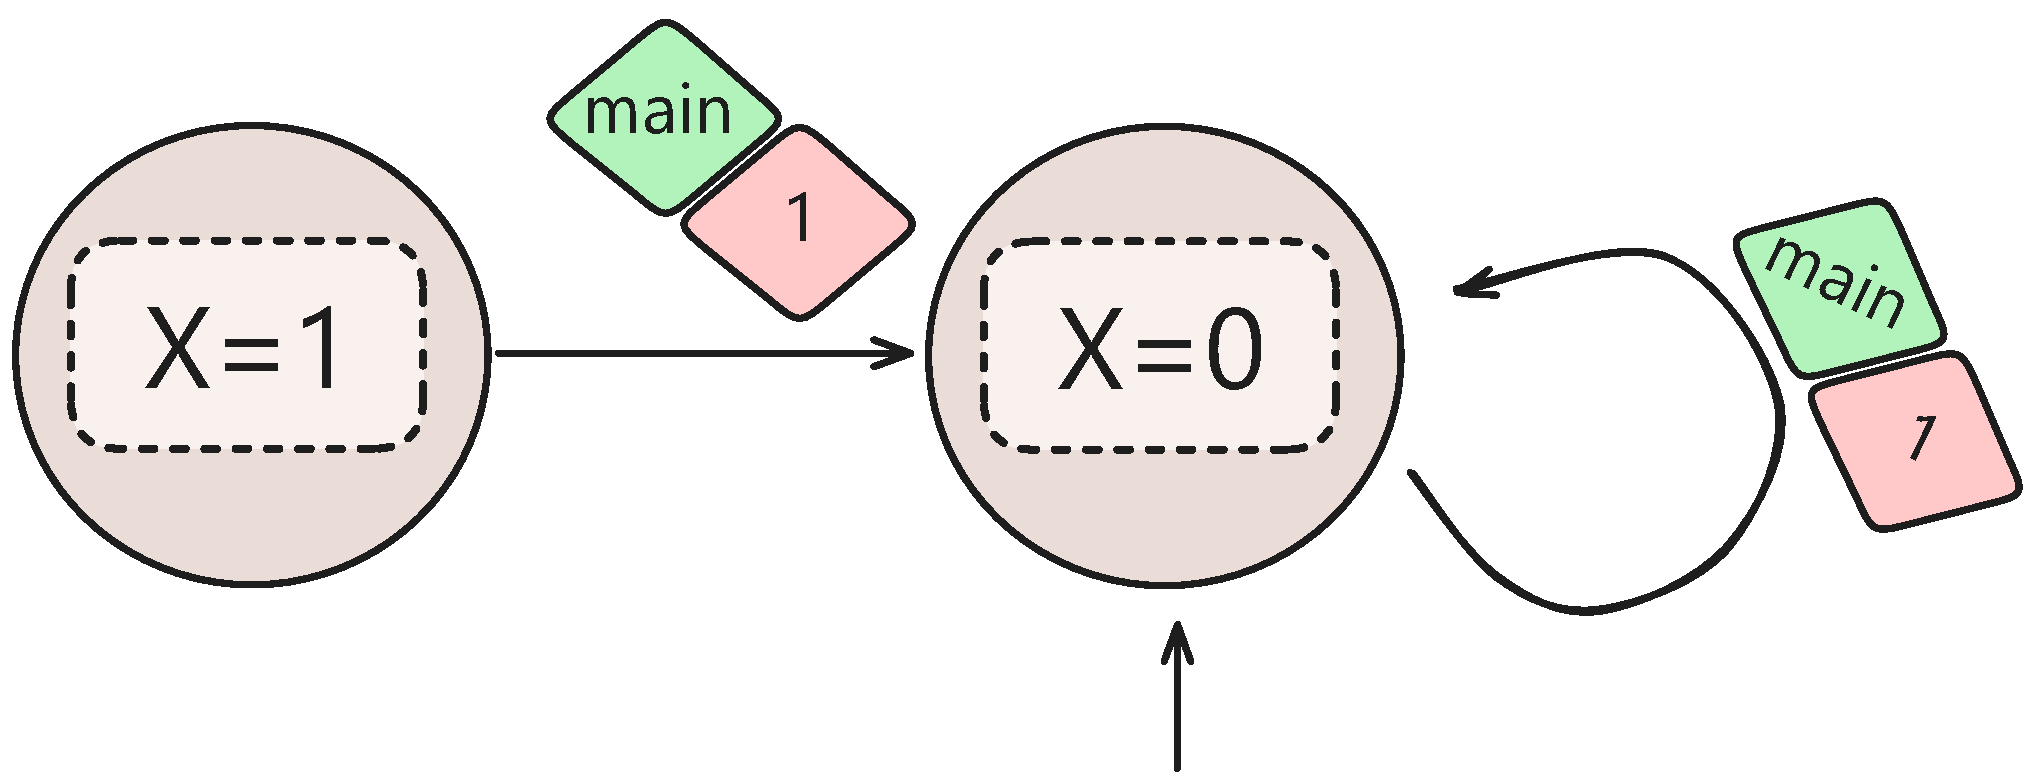
\includegraphics[width=0.48\textwidth,trim=0 0 0 0,clip]{plots/code_2_NFA_v3.pdf}
		
		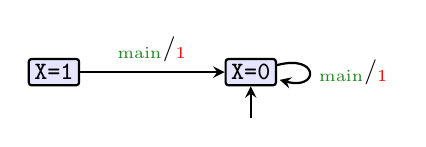
\begin{tikzpicture}[
			->,>=stealth,
			thick,
			node distance=2.5cm,
			state/.style={
				draw=black,
				line width=0.8pt,
				fill=blue!10,
				rectangle,
				rounded corners=1pt,
				inner sep=2pt,
				font=\small
			},
			every node/.style={font=\small}
			]
			% States using the same notation as section 3
			\node[state] (X1) {\texttt{X=1}};
			\node[state, right of=X1] (X0) {\texttt{X=0}};
			
			% Initial state arrow
			\draw[->] ([yshift=-0.4cm]X0.south) -- (X0.south);
			
			% Transitions with proper colored notation from the paper
			\draw[->] (X1) -- node[above] {${\color{ForestGreen}\blacklozenge_{\mathrm{main}}}/{\color{red}\blacklozenge_1}$} (X0);
			\draw[->] (X0) edge[loop right] node[right] {${\color{ForestGreen}\blacklozenge_{\mathrm{main}}}/{\color{red}\blacklozenge_1}$} (X0);
		\end{tikzpicture}
		
		\caption{Serial NFA of Listing~\ref{lst:MotivatingExample2NonSer}.}
		\label{fig:code2ExampleNFA}
	\end{figure}
	
	

	
%	\begin{wrapfigure}{r}{0.50\textwidth}  % “r” = right, width = 0.5\textwidth
%		\centering
%		% 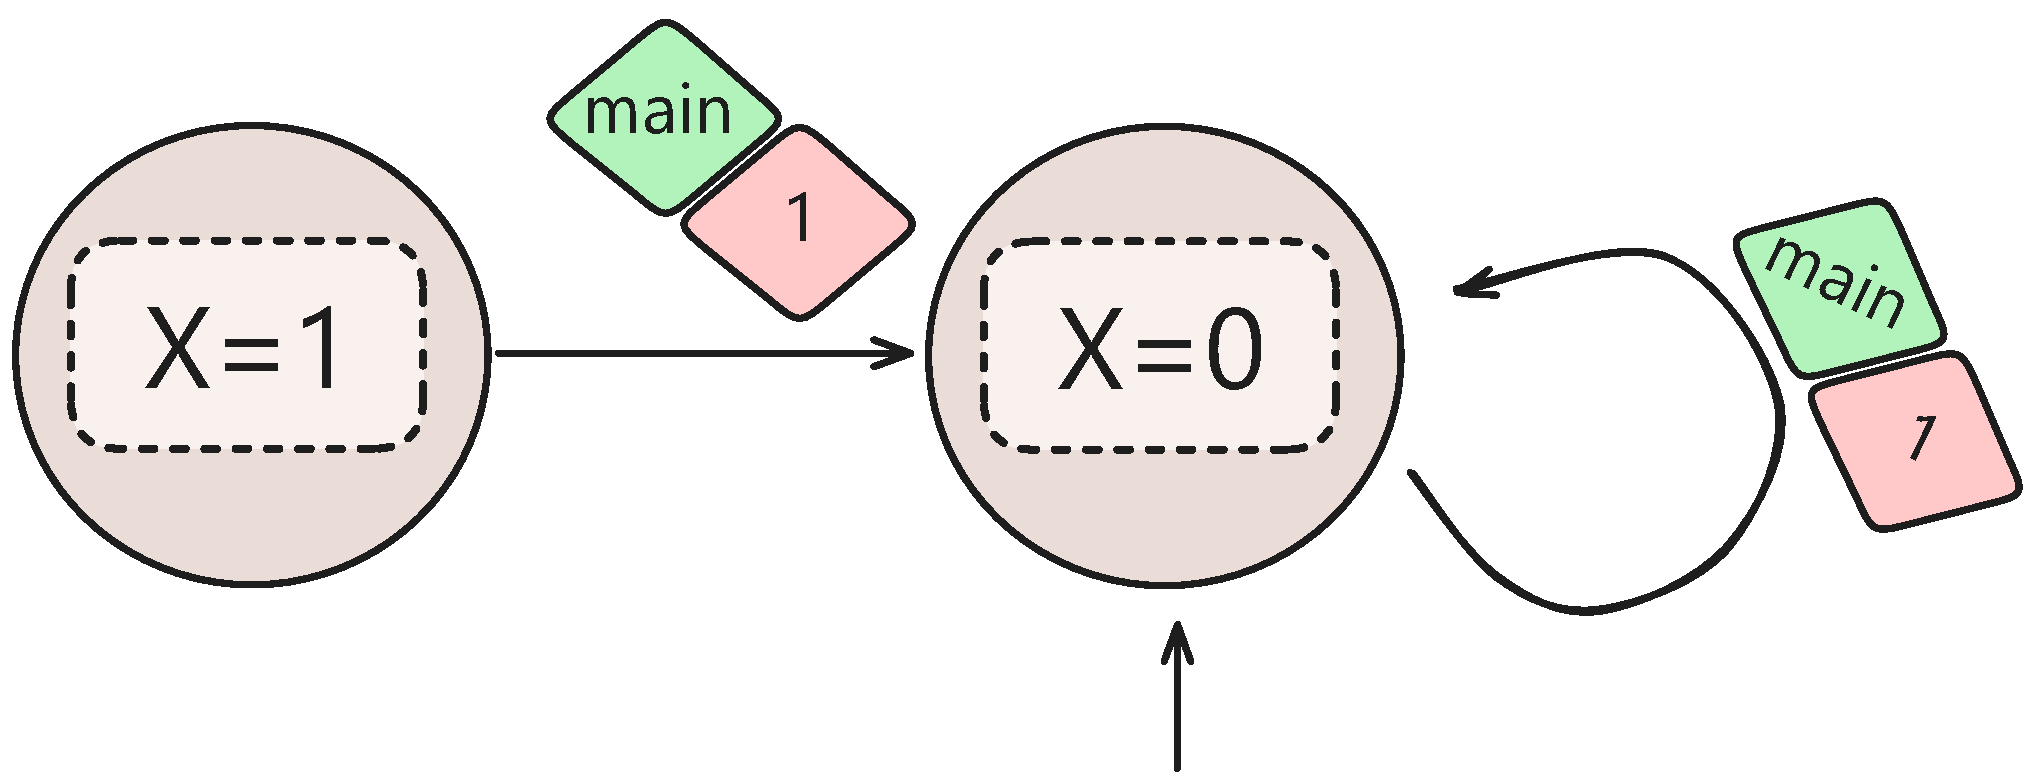
\includegraphics[width=0.48\textwidth,trim=0 0 0 0,clip]{plots/code_2_NFA_v3.pdf}
%		
%		\begin{tikzpicture}[
%			->,>=stealth,
%			thick,
%			node distance=2.5cm,
%			state/.style={
%				draw=black,
%				line width=0.8pt,
%				fill=blue!10,
%				rectangle,
%				rounded corners=1pt,
%				inner sep=2pt,
%				font=\small
%			},
%			every node/.style={font=\small}
%			]
%			% States using the same notation as section 3
%			\node[state] (X1) {\texttt{X=1}};
%			\node[state, right of=X1] (X0) {\texttt{X=0}};
%			
%			% Initial state arrow
%			\draw[->] ([yshift=-0.4cm]X0.south) -- (X0.south);
%			
%			% Transitions with proper colored notation from the paper
%			\draw[->] (X1) -- node[above] {${\color{ForestGreen}\blacklozenge_{\mathrm{main}}}/{\color{red}\blacklozenge_1}$} (X0);
%			\draw[->] (X0) edge[loop right] node[right] {${\color{ForestGreen}\blacklozenge_{\mathrm{main}}}/{\color{red}\blacklozenge_1}$} (X0);
%		\end{tikzpicture}
%		
%		\caption{Serial NFA of Listing~\ref{lst:MotivatingExample2NonSer}.}
%		\label{fig:code2ExampleNFA}
%	\end{wrapfigure}
	%
	%
	%Intuitively, this corresponds to the Listing~\ref{lst:MotivatingExample2NonSer} program updating [X:=1] as an intermediate assignment before yielding.
	
	
	
	\item 
	\textbf{Interleaving Petri Net.}
%	
Next, we translate the NS into a Petri Net \(N_{\mathrm{int}}(\mathcal S)\). The \textit{non-sink places} of the PN represent either (i) global state assignments; and (ii) local states of an in-flight packet. The \textit{sink} places represent request/response pairs of terminating packets.
%
We define the \textit{transitions} between states to correspond to the \(\delta\),\(req\), and \(resp\) mappings of the NS, and with the transitions of the request being able to fire without any input tokens (in order to correspond to initializing arbitrary external requests).
%
Finally, we define the initial marking \(M_0\) to correspond to a single token in the initial global state \(g_0\).
%
This construction (which is fully formalized in Appendix~\ref{appendix:NS-to-PN-formulation}) guarantees that the multiset of all reachable markings \(M\) (with \(M_0 \xrightarrow{}^{*} M\)) projected to the sink places, corresponds to the multiset of all  (${{\color{ForestGreen}\blacklozenge_{\mathit{req}}}/{\color{red}\blacklozenge_{\mathit{resp}}}}$) pairs of the NS, attained by any interleaving, i.e., \(\mathsf{Int}(\mathcal S)\).



\begin{tcolorbox}[colback=black!5!white, colframe=black, boxrule=1pt]
	\textbf{Example.}
%	\textit{Notation.}
In our running example, the NS gives rise to the PN in Fig.~\ref{fig:code2ExamplePN}, encoding all possible interleavings. The places \textcolor{blue}{ $P_2$} and \textcolor{blue}{$P_3$} represent the global states \textcolor{blue}{[X=1]} and \textcolor{blue}{[X=0]}, respectively, while the places $P_1$, $P_4$, $P_5$, and $P_6$ capture the local states of in-flight requests—that is, the remaining program code together with the assignments to each request’s local variables. Similarly, places \textcolor{red}{$P_7$} and \textcolor{red}{$P_8$} correspond to {\color{red}$\blacklozenge_1$} and {\color{red}$\blacklozenge_0$}, respectively, encoding terminated responses. Each token either models an active request, a completed request/response pair, or --- when residing in a global-state place --- the current global state. Finally, transitions implement the network system’s mappings ($\delta/req/resp$): they advance the program by one step, spawn a new request (e.g., transition $t_1$, producing {\color{ForestGreen}$\blacklozenge_{\mathrm{main}}$}), or return a response (e.g., transitions $t_6$ and $t_7$).
\end{tcolorbox}

%Finally, the NS gives rise to the PN in Fig.~\ref{fig:code2ExamplePN}, encoding all possible interleavings.
%%
%The places represent either the global state
%(e.g., places \textcolor{blue}{$P_2$} and \textcolor{blue}{$P_3$} correspond to the global states \textcolor{blue}{[X=1]} and \textcolor{blue}{[X=0]}), while others ($P_1,P_4,P_5,P_6$) correspond to the local state of an in-flight request, i.e., combinations of ``remaining'' programs  assignments to local variables of in-flight requests.
%%
%Furthermore, some requests correspond to responses, e.g., places \textcolor{red}{$P_7$} and \textcolor{red}{$P_8$} corresponds to {\color{red}$\blacklozenge_1$} and {\color{red}$\blacklozenge_0$}.
%%
%Each token corresponds either to a single in-flight request, a single terminated pair of request/response, or (in the case of the global-variable-encoding places), to the current global state.
%%
%Finally, transitions represent the network system's $\delta$ mapping --- encoding either a ``step'' of our program, or spawning a request ($t_1$, which  corresponds to spawning {\color{ForestGreen}$\blacklozenge_\text{main}$}), or returning a response (e.g. transitions $t_6,t_7$).
%


\begin{figure}[!htbp]
	\centering
	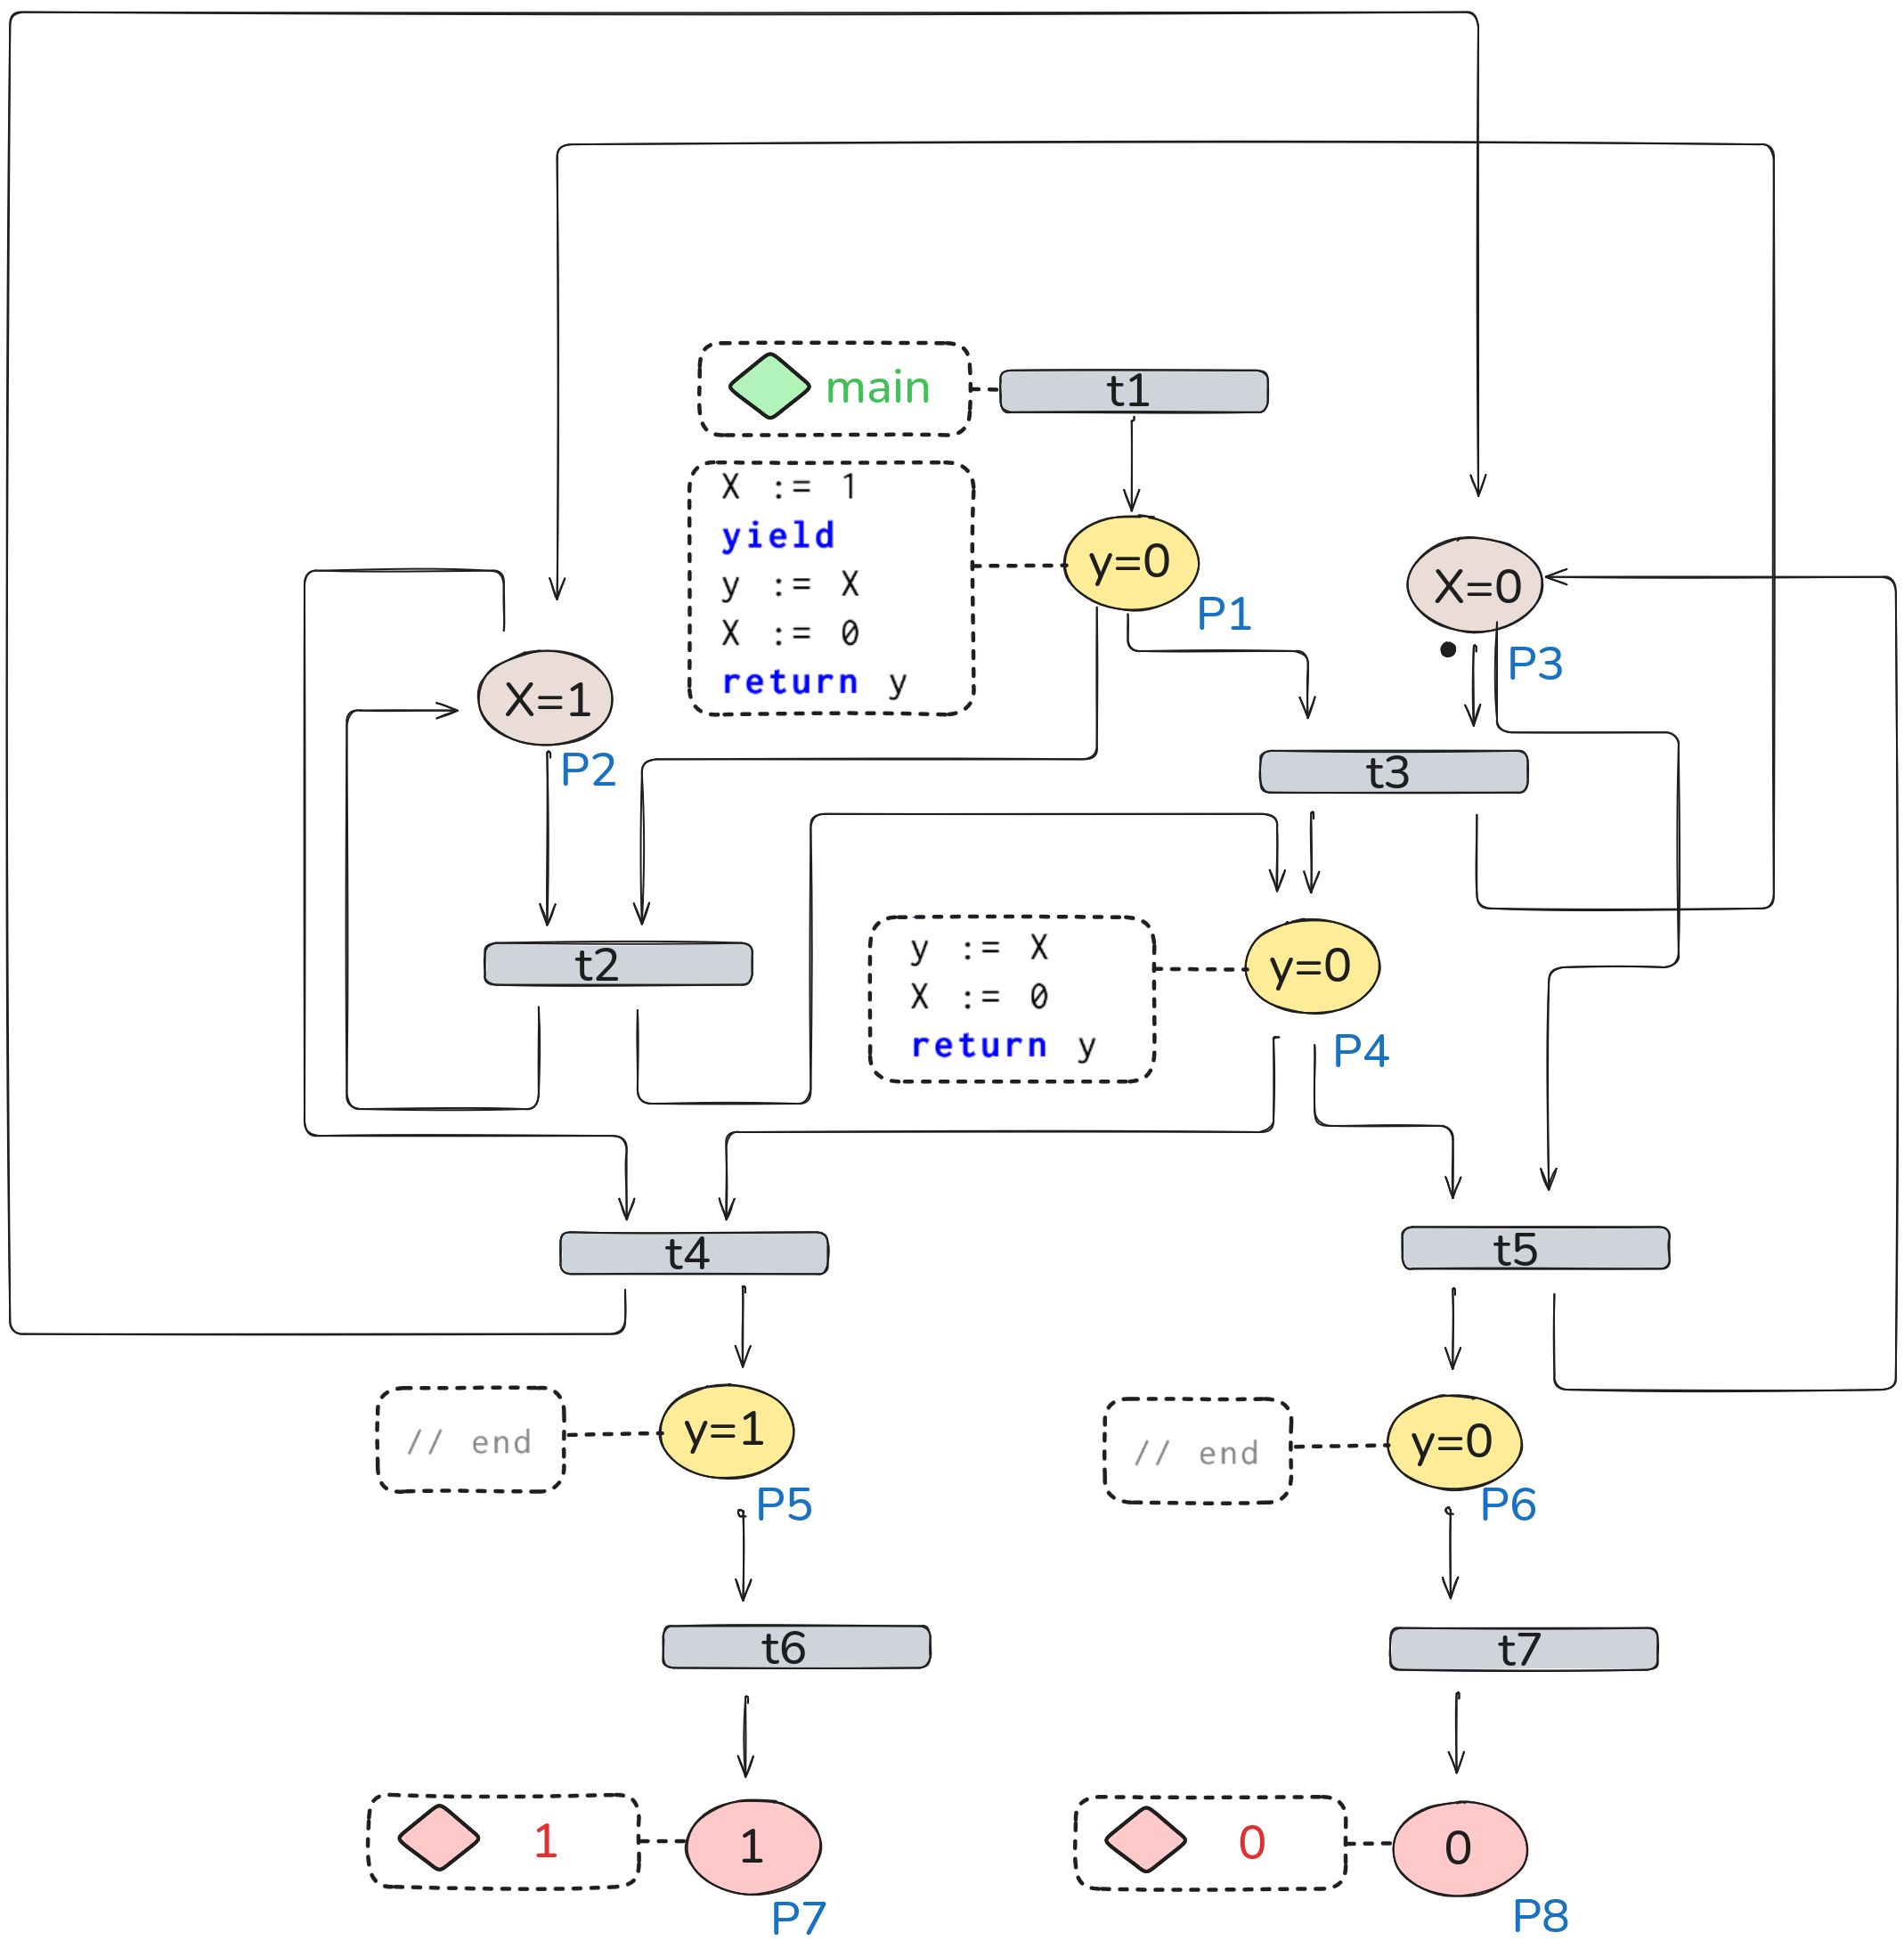
\includegraphics[width=0.7\textwidth]{plots/code_2_PN_with_annotation.png}
	\caption{The PN encoding interleaving executions of the program in Listing~\ref{lst:MotivatingExample2NonSer}.}
	\label{fig:code2ExamplePN}
\end{figure}



	
	
	\item \textbf{Non-serializable set.}  
	Let
	\(\;\mathsf{NonSer}(\mathcal S)=\mathbb N^{|\Sigma|}\setminus \mathsf{Ser}(\mathcal S)\), i.e., all (${{\color{ForestGreen}\blacklozenge_{\mathit{req}}}/{\color{red}\blacklozenge_{\mathit{resp}}}}$) pairs that \textit{cannot} be attained via a serializable execution.
	
	\begin{tcolorbox}[colback=black!5!white, colframe=black, boxrule=1pt]
	\textbf{Example.}
	Regarding the aforementioned program, we automatically generate the following reachability query\footnote{If not for the equality constraints, the problem would have been considered a \textit{coverability} query, which is easier~\cite{Ra78}.} for the Petri net in Figure~\ref{fig:code2ExamplePN}: we encode the target semilinear set by imposing the following constraints on the token distribution:
	%
	%Regarding the aforementioned program, we automatically generate the following reachability query~\footnote{If not the equality constraints, the problem would have been considered a \textit{coverability} query which is easier~\cite{Ra78}.} for the Petri net in Figure~\ref{fig:code2ExamplePN} we encode a target semilinear set with the following constraints on the token distribution:
	%
	\[
	P_1 = 0 \wedge 
	\textcolor{blue}{P_2} \ge 0 \wedge \textcolor{blue}{P_3} \ge 0  \wedge P_4 = 0
	\wedge P_5 = 0 \wedge P_6 = 0 \wedge \textcolor{red}{P_7} \ge 0 \wedge \textcolor{red}{P_8} \ge 1.
	\]
	
	This set encodes all reachable markings with no tokens on $P_1,P_4,P_5,P_6$, at least one token on $\textcolor{red}{P_8}$, and arbitrary tokens on $\textcolor{blue}{P_2},\textcolor{blue}{P_3},\textcolor{red}{P_7}$. 
	\end{tcolorbox} 
	
	
%	\item \textbf{Reachability encoding.}  
	
	
	\item \textbf{Decision \& Validation.}  
	Ask whether there exists a marking \(M\) of \(N_{\mathrm{int}}(\mathcal S)\) such that
	\[
	M_0 \xrightarrow{}^{*} M
	\quad\wedge\quad
	\pi(M)\in \mathsf{NonSer}(\mathcal S).
	\]
	
	\begin{itemize}
		\item [\sat]: yields a counterexample interleaving \(M\) with
		\(\pi(M)\notin \mathsf{Ser}(\mathcal S)\), which is automatically embedded into the NS semantics.
%		We validate a reachable trace and embed it into the NS semantics, yielding a valid interleaving that produces request/response pairs unattainable under any serial execution.
		
		\item [\unsat]: yields an inductive invariant of
		\(N_{\mathrm{int}}\), which back-translates to a proof of
		serializability 
		for \(\mathcal S\),
		%
		validated by synthesizing an inductive invariant over the interleaving PN, thereby proving that the corresponding semilinear set cannot be realized by any interleaving (see Appendix~\ref{appendix:ns-serializable}).
	\end{itemize}

\begin{tcolorbox}[colback=black!5!white, colframe=black, boxrule=1pt]
	\textbf{Example.}
	This target semilinear set of markings is, in fact non-empty. For example, it includes the following reachable marking:
	
	\[
	M^* = \{\textcolor{blue}{P_3}(1),\;\textcolor{red}{P_7}(1),\;\textcolor{red}{P_8}(1)\}
	\]
	
	Table~\ref{tab:PetriNetFiringCounterexample} (in Appendix~\ref{appendix:non-serializable-execution-example}) lists a valid firing sequence that leads to a satisfying marking $M^*$ from the initial state.
	%
%	As the target set encodes request/response pairs that are \textit{unattainable} via serial executions, and as the PN encodes all possible interleavings, this firing sequence also corresponds as a counterexample demonstrating the program is non-serializable. 
	%
	Specifically, the reachable marking encodes the outputs $\{{\color{ForestGreen}\blacklozenge_\text{main}}/{\color{red}\blacklozenge_0},{\color{ForestGreen}\blacklozenge_\text{main}}/{\color{red}\blacklozenge_1}\}$ which are indeed attained only via a non-serializable execution (see Sec.~\ref{sec:introduction}).
\end{tcolorbox} 
%\item \textbf{Validation.}  
%
%	\begin{itemize}
%		
%		\item[\sat]: 
%		See the example in subsec.~\ref{subsec:ns-not-serializable}.
%		
%%		\item[\unsat]: 
%		
%		
%	\item \sat: we validate the reachable trace and project it to the NS semantics to represent a valid interleaving that results into request/response pairs which cannot be attained in serial executions.
%	See example in subsec.~\ref{subsec:ns-not-serializable}.
	
%	\item \unsat:
%	we generate an inductive invariant over the interleaving PN, proving that the semilinear set cannot be attained via an interleaving.
%	See example in subsec.~\ref{subsec:ns-serializable}.
%\end{itemize}

\end{enumerate}

\medskip
\noindent
\textbf{Complexity Analysis.}
The core algorithm reduces serializability checking to Petri net reachability with semilinear target sets. 
Since the serial executions form a regular language (step 1), their Parikh Image is effectively semilinear by Parikh's theorem, with size exponential in the NFA.
The interleaving Petri net (step 2) has $O(|G| + |L| + |\mathit{REQ}| \times |\mathit{RESP}|)$ places and $O(|\mathit{REQ}| + |\delta| + |\mathit{RESP}|)$ transitions.
The reachability query (step 3) asks whether the Petri net can reach the complement of a semilinear set, which is decidable but Ackermann-complete~\cite{CzWo22}.
Without optimizations, even simple examples can generate Petri nets with hundreds of places and exponentially-sized semilinear constraints, making the approach impractical.
Our optimizations (Section~\ref{sec:optimizations}) dramatically reduce both the Petri net size and the semilinear set complexity.


%\guy{should we add/prove the following?}
%
%\begin{proposition}
%	Let $N_{\mathrm{int}}(\mathcal S)=(P,T,\mathsf{pre},\mathsf{post},M_0)$ be the interleaving Petri net constructed above, and let
%	\[
%	\pi\colon\mathbb N^P\to\mathbb N^{P_R}
%	\]
%	be the projection onto the request/response places $P_R$.  Then
%	\[
%	\mathsf{Int}(\mathcal S)
%	\;=\;
%	\{\;\pi(M)\;\mid\;M_0\xrightarrow{*}M\}.
%	\]
%\end{proposition}


\subsection{Optimizations}
\label{sec:optimizations}

%\todo{check}

We apply four optimizations to the base algorithm to control intermediate blow‐up in the size of both the PN and the constructed semilinear set. 
%
An extensive empirical evaluation of these optimizations appears later on in subsec.~\ref{subsec:optimization-results}.

\medskip
\noindent
\textbf{(1) Bidirectional pruning.}  
When solving Petri net reachability, many places and transitions might be irrelevant to the specific target set.  
	We prune them before symbolic reasoning by combining forward and backward passes:  
	the forward pass over-approximates the places reachable from $M_0$; and symmetrically,   
	the backward pass traverses in reverse from any place that can influence a target constraint (hence over-approximating the places that can contribute to it).
	We iteratively remove non-forwards-reachable and
	non-backwards-relevant places and transitions, to a fixed point.  
	Appendix~\ref{appendix:BidirectionalProof} illustrates this (Fig.~\ref{fig:bidirectional_pruning}) and proves soundness (Theorem~\ref{thm:bidirectional-pruning}):


%\guy{check with mark (M0 projected on P or P'?)}

\begin{theorem}[Bidirectional Pruning Soundness]
	\label{thm:bidirectional-pruning}
	Let $N = (P, T, Pre, Post, M_0)$ be a Petri net and $S$ a target set.  
	Let $N' = (P',T',\,\Pre|_{P'\times T'},\,\Post|_{P'\times T'},\,M_0|_{P})$ be the pruned net.  
	Then $S$ is reachable from $N$ iff it is reachable from from $N'$.
\end{theorem}
%
%We depict this in Fig.~\ref{fig:bidirectional_pruning}, and prove Theorem~\ref{thm:bidirectional-pruning} in Appendix~\ref{appendix:BidirectionalProof}.
% (see the proof in Appendix~\ref{appendix:BidirectionalProof}).
%

% \medskip
% \noindent\textit{\textbf{Intuition.}}
% Before any heavy symbolic reasoning takes place, we apply bidirectional pruning on the underlying PN.  In the forward pass, we traverse from the initial marking to identify an over-approximation of all places and transitions that could ever fire; in the backward pass, we traverse backward from any place that can influence a target constraint, and identify over-approximations on transitions and places that cannot contribute to reaching it.  By iteratively repeating forward passes and backward passes until convergence, we remove every component of the net that cannot both originate and contribute to the reachable target set.  This dramatically shrinks the net in practice, often converting an intractably large model into one small enough for exhaustive analysis.

\medskip
\noindent
\textbf{(2) Semilinear set pruning.}  
A semilinear set $S=\bigcup_{i=1}^m L_i$ with 
	$L_i=\{\,b_i+\sum_{p\in P_i}n_p p \mid n_p\in\mathbb N\}$ may contain redundant 
	period vectors or components.  
	We prune during construction:
	(1) remove any $p\in P_i$ expressible as a nonnegative combination of $P_i\setminus\{p\}$, 
	and (2) drop $L_i$ when $L_i\subseteq L_j$.  
	This keeps formulas compact and solver calls tractable.




% it is common for some inequalities or disjuncts to add no new coverage beyond what other constraints already guarantee.  The redundant‐constraint elimination pass inspects each linear inequality and each disjunct in a disjunctive normal form, testing whether it is implied by the rest.  Any constraint or disjunct found redundant is dropped, ensuring that subsequent intersection, union, and projection operations work on the smallest necessary formula.  This streamlines the logic formula and prevents unnecessary size blow‐ups during solver invocations.

% %
% We replace each period‐basis \(P_i\) by
% \[
% P_i \;:=\;\{\,p\in P_i \mid p\notin\mathsf{Span}(P_i\setminus\{p\})\}
% \],
% Dropping any ``redundant'' periods, and removing any \(L_j\subseteq L_i\) for \(i\neq j\), iterating to a fixed point so no two components subsume one another.

\medskip
\noindent
\textbf{(3) Generating fewer constraints.}  
When computing the Parikh Image of a regular expression as a semilinear set,
	most regex operations can be implemented without an exponential blow-up.
	However, Kleene star is a notable exception: in the general case, it can cause and exponential blow up: for $S=\bigcup_{i=1}^m L_i$,  the Kleene star $S^\ast$ is given as a semilinear set by: 
	\[
	S^\ast=\bigcup_{I \subseteq \{1,...,m\}} 
	\Big\{\sum_{i \in I} b_i + \sum_{p \in \bigcup_{i \in I} P_i\cup \{b_i\}} n_p p\Big\}.
	\]
	This yields $2^m$ components. To mitigate:
	(i) if $L_i=\{b_i\}$ (period-less component), factor it out, star the rest, then add $b_i$ as a period;  
	(ii) if $L_i=\{\sum_{p\in P_i}n_pp\}$ (zero base), likewise star the rest and add each $p\in P_i$.  
	Each such case halves the component count, giving exponential savings.




% Let $\mathrm{comp}(S)=\{L_1,\dots,L_m\}$ 
% be the multiset of linear components of the semilinear set 
% \(\displaystyle S=\bigcup_{i=1}^m L_i\), where each 
% \(\;L_i=b_i+\langle P_i\rangle\) with \(b_i\in\mathbb N^d\) and 
% \(P_i\subseteq\mathbb N^d\).  Define the pruning operator
% \[
% \mathrm{new}(\mathcal C)
% \;=\;
% \bigcup\bigl\{\,L\in\mathcal C \;\bigm|\;\nexists\,L'\in\mathcal C\setminus\{L\}:\;L'\subsetneq L\bigr\},
% \]
% which removes any component strictly containing another.  
% %
% \guy{Nicolas is it clear we mean that we fix their semilinear "meaning" of the regex operations? For example, + is union etc..}
% Then, we replace the naive semilinear‐set operations by
% \[
% S\;+\;T
% \;=\;
% \mathrm{new}\bigl(\mathrm{comp}(S)\,\cup\,\mathrm{comp}(T)\bigr),
% \]
% \[
% S\;\cdot\;T
% \;=\;
% \mathrm{new}\Bigl(\{\,L_i\cdot L'_j \mid L_i\in\mathrm{comp}(S),\;L'_j\in\mathrm{comp}(T)\}\Bigr),
% \]
% where for
% \(\;L_i=b_i+\langle P_i\rangle,\;L'_j=b'_j+\langle P'_j\rangle\) we set
% $
% L_i\cdot L'_j
% =\;(b_i+b'_j)\;+\;\langle\,P_i\cup P'_j\,\rangle.
% $
% Finally, for Kleene‐star and plus on the regex side one similarly applies
% \(\mathrm{new}(\cdot)\) to the collection of ``folded” components instead of
% building all intermediate ones:
% \[
% S^*
% =\mathrm{new}\Bigl(\bigcup_{k\ge0}\bigl(\mathrm{comp}(S)\bigr)^k\Bigr),
% \qquad
% S^+
% =S\cdot S^*.
% \]

% \medskip
% \noindent\textit{\textbf{Intuition.}}
% %
% During set construction --- especially when introducing new existentially‐quantified variables or combining transition effects, we selectively avoid generating any marking that would strictly dominate an already‐seen solution.  In effect, whenever a candidate disjunct would yield a superset of an existing one, it is skipped entirely.  This ``generate‐less” heuristic stops the proliferation of large, overlapping regions in the semilinear description.  In benchmarks with large state spaces, it can reduce the number of intermediate branches by orders of magnitude.

\medskip
\noindent
\textbf{(4) Strategic Kleene elimination order.}  
The size of the generated semilinear set is not only impacted by how the
	semilinear set operations are implemented, but also by what specific regular
	expression is given as input: a single regular language may be represented by a
	number of equivalent regexes, each of different complexity.
	%
	In particular, as Kleene star can cause a large blow-up in the semilinear set size,
	we are especially sensitive to the \emph{star height} of the generated regex.
	%
	Naive Kleene elimination may introduce many nested stars.  
	We reduce this by strategically choosing the next state to eliminate by:
	\[
	q^*=\arg\min_{q\in Q'}\bigl(|\delta_{\mathrm{in}}(q)|+|\delta_{\mathrm{out}}(q)|\bigr),
	\]
	eliminating lower-degree states first.  
	This heuristic empirically yields smaller regexes and more compact semilinear sets.


%\medskip
%\noindent
%\textbf{(4) Strategic Kleene elimination order.}  
%The size of the generated semilinear set is not only impacted by how the
%semilinear set operations are implemented, but also by what specific regular
%expression is given as input: a single regular language may be represented by a
%number of equivalent regexes, each of different complexity.
%%
%In particular, as Kleene star can cause a large blow-up in the semilinear set size,
%we are especially sensitive to the \emph{star height} of the generated regex.
%%
%We use Kleene's algorithm to convert an NFA $\mathcal A=(Q,\Sigma,\delta,q_0,F)$ to a regex, which works by repeated state elimination, choosing one state at a time.
%Naively, when eliminating states in an arbitrary order, Kleene's algorithm may generate regexes with a much greater star height than necessary---a problem
%when converting to semilinear sets.
%%
%Therefore, we heuristically optimize the state elimination order to end up with a smaller regex. Formally, we pick the next state:
%\[
%q^* = 
%\arg\min_{q\in Q'}\bigl(|\delta_{\mathrm{in}}(q)|+|\delta_{\mathrm{out}}(q)|\bigr)
%\]
%where \(Q'\subseteq Q\) are the states remaining to be eliminated, choosing to
%eliminate states with a smaller total degree first.
%%
%This empirically keeps the resulting regexes small.

% \medskip
% \noindent\textit{\textbf{Intuition.}}
% When converting an NFA to a single regex, we pick the next state to eliminate by heuristically choosing the  state with the fewest incoming and outgoing edges.
% This optimization allows for circumventing 
% overblown expressions resulting in naive translations, especially with regard to  Kleene closures (the “\(\mathsf{*}\)” operator).  Instead, we analyze the structure of sub-expressions under the various operators --- estimating their branching factor, and reordering them so that simpler, low‐branching components are expanded first.  
%This adaptive ordering often leads to early detection of fixed points or dead‐ends, preventing the combinatorial explosion that arises when complex loops are expanded prematurely.  



\section{Implementation}
\label{sec:implementation}
\begin{wraptable}[11]{r}{0.32\textwidth}
	\vspace{-1.5em} 
	\centering
	\begin{tabular}{@{} l S[table-format=5.0] @{}}
		\toprule
		\textbf{Module}                & {\textbf{LoC}} \\
		\midrule
		Input \& Parsing               &  1723          \\
		Model Construction             &  5561          \\
		Petri–Net Conversion           &   843          \\
		Reachability          &  2628          \\
		Proof Checking                 &  3240          \\
		Utilities                      &  2160          \\
		Testing \& Evaluation          &  2118          \\
		\midrule
		\textbf{Total}                 & \textbf{18273} \\
		\bottomrule
	\end{tabular}
	\caption{Lines of Code}
	\label{tab:loc_summary2}
\end{wraptable}

We implemented our approach in \toolname{}~\cite{ArtifactRepository}, a publicly available tool consisting of over $18{,}200$ LoC written mostly in \texttt{Rust} (see Table~\ref{tab:loc_summary2}).
%
%We next elaborate on the architecture of our tool and the various optimizations we added to allow it to run efficiently.
%
%For the underlying Petri Net model checker, we use SMPT~\cite{AmDa23} which supports \textit{unbounded} reachability queries (see Appendix~\ref{appendix:smpt}).
%, and which uses Z3 as an underlying SMT solver~\cite{DeBj08}. 
%and which we extended to support our setting (for example, we needed to extend the solver to support proof generation). 
%
%We note that other off-the-shelf solvers can be used as well.

%The implementation..

%\begin{enumerate}
%	\item The extra things we did to make the thing actually run
%	\item Code architecture
%	\item Optimizations
%\end{enumerate}

%\newpage
\subsection{Code Architecture}

%\begin{tabular}{|l|r|}
%	\hline
%	\textbf{Module} & \textbf{LoC} \\
%	\hline
%	Input \& Parsing                             & 1723  \\
%	\hline
%	Model Construction                           & 5561  \\
%	\hline
%	Petri-Net Conversion                         & 843   \\
%	\hline
%	Reachability Checking                        & 2628  \\
%	\hline
%	Proof Checking                               & 3240  \\
%	\hline
%	Utilities                                       & 2160  \\
%	\hline
%	Testing \& Evaluation               & 2118  \\
%	\hline
%	\textbf{Total}                               & \textbf{18273} \\
%	\hline
%\end{tabular}


%
%\begin{table}[ht]
%	\centering
%	\label{tab:loc_summary}
%	\begin{tabular}{@{} l S[table-format=5.0] @{}}
%		\toprule
%		\textbf{Module}                & {\textbf{LoC}} \\
%		\midrule
%		Input \& Parsing               &  1723          \\
%		Model Construction             &  5561          \\
%		Petri–Net Conversion           &   843          \\
%		Reachability Checking          &  2628          \\
%		Proof Checking                 &  3240          \\
%		Utilities                      &  2160          \\
%		Testing \& Evaluation          &  2118          \\
%		\midrule
%		\textbf{Total}                 & \textbf{18273}          \\
%		\bottomrule
%	\end{tabular}
%	\caption{Lines of Code by Module}
%\end{table}
%

% Then, where you want the table wrapped to the right:
%
% this table summarizes the values without whitespaces/comments and without the code for SMPT (or the wrapper) or the carfo and toml files
%
%\begin{wraptable}[8]{r}{0.32\textwidth}
%	\centering
%	\begin{tabular}{@{} l S[table-format=5.0] @{}}
%		\toprule
%		\textbf{Module}                & {\textbf{LoC}} \\
%		\midrule
%		Input \& Parsing               &  1723          \\
%		Model Construction             &  5561          \\
%		Petri–Net Conversion           &   843          \\
%		Reachability          &  2628          \\
%		Proof Checking                 &  3240          \\
%		Utilities                      &  2160          \\
%		Testing \& Evaluation          &  2118          \\
%		\midrule
%		\textbf{Total}                 & \textbf{18273} \\
%		\bottomrule
%	\end{tabular}
%	\caption{Lines of Code (LoC)}
%	\label{tab:loc_summary2}
%\end{wraptable}
%
%\noindent
%
\toolname{} implements an end-to-end serializability checker for a given input program. If the program is serializable, we return a proof thereof; otherwise, if it is not serializable, a counterexample is given to the user for an interleaving that can result in request/response pairs that are unattainable in any serial execution.
%
Our workflow translates the decidability problem to an equivalent Petri Net reachability question (for unbounded nets), in which (i) the Petri Net represents all possible interleavings of the problem; and (ii) the reachability query represents a semilinear set (equivalently, a Presburger arithmetic encoding) of all request/response pairs that cannot be attained in any serial execution.
%
As Petri Net reachability is Ackermann-complete~\cite{CzWo22}, we added various optimizations to expedite the search process, both at the PN level and the property-encoding level.
%
The pipeline of \toolname{} is depicted in Fig.~\ref{fig:full_program_flow}, and includes:
 

\begin{enumerate}
	\item \textbf{Input \& Parsing.} 
	Our framework receives either a \texttt{SER} program with the syntax described in Sec.~\ref{sec:problem-definition}; or a \texttt{JSON} file directly encoding a network system. In the case of the former, an additional step takes place, parsing the input %(using the \texttt{parser.rs} module) 
	to an expression tree that is translated to an equivalent NS.
%	, represented as a struct in the \texttt{ns.rs} module. 
	
	\item \textbf{Petri Net Conversion.} The NS is then translated into a Petri Net 
%	(see the \texttt{petri.rs} module) 
which represents the interleavings. 
%	.as depicted, for example, in subsec.~\ref{subsec:ns-not-serializable}.
%	Each place represents a state (either global or local) or a response. Each token represents a single in-flight request or a terminated response. 
The PN is encoded in the de-facto standard \texttt{NET} format, to support off-the-shelf PN model checkers. 
	
	\item \textbf{Semilinear Conversion.} 
%	This includes a set of modules (\texttt{kleene.rs}, \texttt{semilinear.rs}, and \texttt{presburger.rs}) which 
These modules generate a semilinear set encoding all non-serializable outputs, via translation of the serialized NFA (e.g., Fig.~\ref{fig:code2ExampleNFA}) to a regex, which is then projected (via the Parikh Image) and complemented. 
%	This conversion is done by the following pipeline: (1) the NS is translated to an NFA encoding all possible request/response pairs of the input program; (2) This NFA is translated to a regex (via Kleene's Theorem) and then projected (via the Parikh Image) to a semilinear set. The (finite) encoding of the semilinear set symbolically represents all outputs attained via serializable executions of the program, running for an unbounded number of steps; (3) finally, we complement the semilinear set to encode all outputs unattainable via serial executions. 
	At the end of the pipeline, an \texttt{XML}-formatted output encodes a reachability query that encapsulates constraints over the PN token count.
	
	
	\item \textbf{Reachability Engine.} The PN and the reachability query are fed to a  PN model checker, which runs \textit{Bounded Model Checking} (BMC)~\cite{BiCiClZh99} in search of a counterexample; and \textit{state equation reasoning}~\cite{Mu77} in order to prove non-reachability. 
%	This engine is implemented in the \texttt{reachability.rs} and \texttt{reachability\_with\_proofs.rs}  modules.
	%
	In order to expedite the search, ``large'' (PN, query) pairs are replaced with multiple pruned PNs (generated by the reachability engine), each coupled with a sub-query encoding a separate disjunct. 
%	of the original query.
%	We iteratively solve the 
The disjuncts are solved on the fly, until reaching \texttt{SAT}, in which case, we have a counterexample; otherwise, if all disjuncts are \texttt{UNSAT}, we render the original program as serializable.
	
	
	\item \textbf{Proof \& Certificate Handling.} If the query is \texttt{SAT}, we reconstruct a non-serializable NS-level execution and validate its correctness. Otherwise, if all disjuncts are \texttt{UNSAT}, our proof module extracts a separate proof for each disjunct. We subsequently ``stitch'' these proofs to a single inductive invariant, and project it to the NS-level, representing a full inductive proof certificate for serializability. Our checker also validates that the inductive invariant is correct, i.e., (i) includes the initial state; (ii) is inductive with regard to the transitions; and (iii) implies that the reachability query is \texttt{UNSAT}.
	%, and hence, implying serializability. 
	
	
	\item \textbf{Instrumentation \& Logging.} Throughout the pipeline, intermediate representation and performance metrics 
%	input size and performance metrics (number of places, transitions, constraint complexity, timings) 
are recorded. 
%The logger outputs 
%We generate \texttt{CSV} and \texttt{JSON} logs along with
% analysis. 
	%
%	We also assemble 
%an \texttt{HTML} report embedding the original net, symbolic constraints, reachability results, proofs, etc.
%	\item \textbf{Debug Report Generation.} Finally, a human-readable \texttt{HTML} report is assembled: it embeds the original net, symbolic constraints, reachability results, proof outlines, and profiling graphs. This interactive report allows users to drill down into each transition firing, constraint check, and proof obligation.
	
%	\item \textbf{Output Delivery.} The crate exposes a simple CLI and library API. Users obtain either a Boolean reachability verdict (with optional certificate), raw log files, or a full HTML debug report, depending on invocation flags.
	
%	\item \textbf{Optimizations.} As formalized in the previous section, we implement multiple optimizations throughout the process.
%	, both for representing the semilinear sets succinctly and for pruning the Petri Nets. These optimizations significantly reduce the search space and expedite the model-checking process.
\end{enumerate}



%\noindent
%This linear pipeline - \emph{parse} -> \emph{model} -> \emph{normalize} -> \emph{analyze} -> \emph{prove} -> \emph{report} --- ensures a clear separation of concerns, easy extensibility (e.g., swapping backends), and comprehensive traceability from input to certified result.```


\begin{figure}[!htbp]
	\centering
	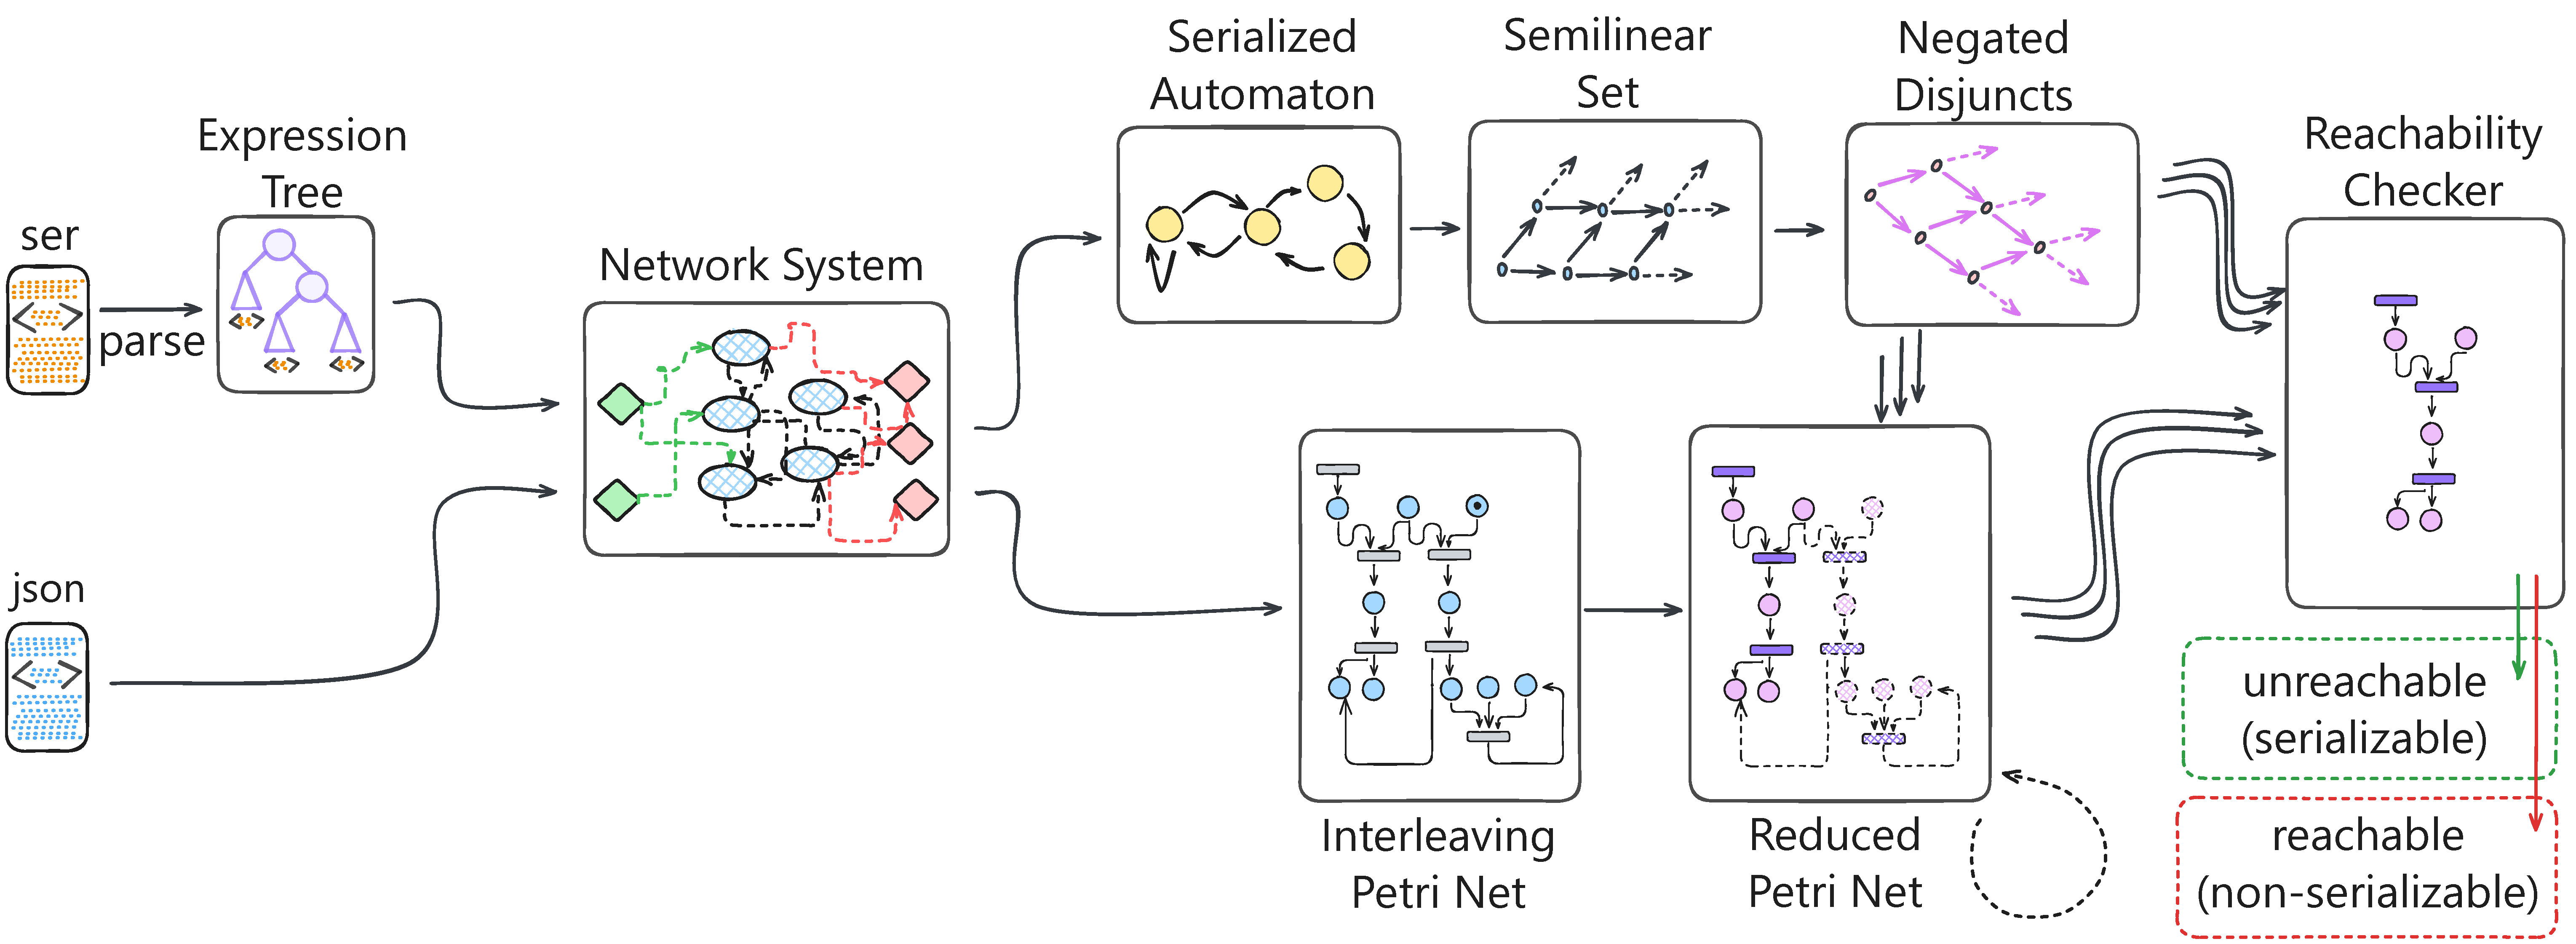
\includegraphics[width=1.0\textwidth]{plots/full_program_flow.pdf}
	\caption{Full program flow 
%		If the target set is unreachable --- a serializability proof is produced; otherwise, if it is reachable --- a counterexample trace is generated.
	(simplified, without backward arrows 
%	translating invariants (if serializable) or counterexample traces (if non-serializable) back 
	to the NS level).}
	\label{fig:full_program_flow}
\end{figure}


%\subsection{Optimizations}

%\paragraph{Bidirectional Pruning of the Petri Net}
%Before any heavy symbolic reasoning takes place, we apply bidirectional pruning on the underlying PN.  In the forward pass, we traverse from the initial marking to identify all places and transitions that could ever fire; in the backward pass, we traverse backward from any place that can influence a target constraint, and identify transitions and places that cannot contribute to reaching it.  By iteratively repeating forward passes and backward passes until convergence, we remove every component of the net that cannot both originate and contribute to the reachable target set.  This dramatically shrinks the net in practice, often converting an intractably large model into one small enough for exhaustive analysis.
%%
%We depict this in Fig.~\ref{fig:bidirectional_pruning}, and give a formal proof of correctness in Appendix~\ref{appendix:BidirectionalProof}.

%\paragraph{Redundant‐Constraint Elimination}
%When manipulating Presburger sets or their semilinear representations, it is common for some inequalities or disjuncts to add no new coverage beyond what other constraints already guarantee.  The redundant‐constraint elimination pass inspects each linear inequality and each disjunct in a disjunctive normal form, testing whether it is implied by the rest.  Any constraint or disjunct found redundant is dropped, ensuring that subsequent intersection, union, and projection operations work on the smallest necessary formula.  This streamlines the logic formula and prevents exponential blow‐up of case distinctions during solver invocations.
%
%Every time you build or star a semilinear set, you prune out any “period” vectors that are rendered useless by earlier steps:. nce you’ve accumulated a bunch of LinearSet components, you try to merge any that mathematically subsume one another:

%\paragraph{Generating Fewer Constraints}
%During set‐construction--- especially when introducing new existentially‐quantified variables or combining transition effects, we selectively avoid generating any marking that would strictly dominate an already‐seen solution.  In effect, whenever a candidate disjunct would yield a superset of an existing one, it is skipped entirely.  This ``generate‐less” heuristic stops the proliferation of large, overlapping regions in the semilinear description, trading off completeness of intermediate case‐enumeration for concise final representations.  In benchmarks with large state‐spaces, it can reduce the number of intermediate branches by orders of magnitude.

%in both the Regex and SemilinearSet Kleene-algebra instances. Concretely, instead of always building the full new structure and pruning it later, operations like union (plus) and concatenation (times) do a quick check for trivial cases and drop “zero” or “one” elements on the spo

%\paragraph{Executing Kleene Elimination in a Strategic Order:}
%When converting an NFA to a single regex, we pick the next state to eliminate by heuristically choosing the  state with the fewest incoming and outgoing edges.
%This optimization allows circumventing 
%overblown expressions resulting in naive translations, especially with regard to  Kleene closures (the “\(\mathsf{*}\)” operator).  Instead, we analyze the structure of sub-expressions under the various operators --- estimating their branching factor, and reorder them so that simpler, low‐branching components are expanded first.  This adaptive ordering often leads to early detection of fixed points or dead‐ends, preventing the combinatorial explosion that arises when complex loops are expanded prematurely.  




\subsection{Benchmark Overview} 
\label{subsec:benchmarks}
To the best of our knowledge, ours is the first and only tool to: (i) statically check serializability on \textit{unbounded} programs; and (ii) \textit{prove serializability holds}.
%
Thus, and due to lack of standard benchmarks for evaluating serializability, we 
assembled a suite of dozens of benchmarks (accompanying our artifact~\cite{ArtifactRepository}).
These include both serializable and non-serializable instances encoded in both \texttt{SER} and \texttt{JSON} formats, and covering a broad range of features, including arithmetic, locks, loops, non-determinism, and more (see an overview of all our benchmarks in Table~\ref{tab:benchmarks-all} of Appendix~\ref{appendix:full_results}.
%
We note that although the benchmarks themselves are not the main part of the paper, we believe they have merit on their own, due to their relevance to various real-world systems of interest.
%
Specifically, we wish to note our suite of benchmarks encoding \textit{networking \& system protocols} (see Table~\ref{tab:networking-benchmarks}), which include stateful firewalls, BGP routing programs, network monitors, and more --- 
%highlighting the serializability challenges inherent in real-world distributed programs.
%
%Here, we were motivated by 
as motivated by real-world concurrency problems in this domain. One such example is our \textit{routing-cycle benchmark} in software-defined networks, (motivated by~\cite{NaGhSa24}). Another real-world example is our \textit{snapshot isolation benchmark} (explained in Appendix~\ref{appendix:tour}), that was motivated by a real database bug, namely, duplicate-key errors~\cite{cockroach-issue-14099} in the \texttt{CockroachDB} system~\cite{cockroachdb-si-docs}, and the non-serializable behavior was automatically identified by our toolchain.
%
%Our benchmarks include both serializable and non-serializable instances, and their features and categorization appears in Table~\ref{tab:benchmarks-all}. 



%As there are no standard benchmarks for evaluating serializability, we wrote dozens of programs in our abstract NS language. These benchmarks span a wide range of complexity --- covering branching, looping constructs, arithmetic, non-deterministic choice, and multi-request workflows that manipulate both shared (global) variables and per-request (local) state. 
%
%We include both serializable and non-serializable instances and summarize the benchmarks' features and categorizations in Table~\ref{tab:benchmarks-all}. 
%
%In particular, our most sophisticated examples are drawn from realistic networking and system-protocol scenarios, including stateful firewalls, BGP routing, network monitoring, and more --- highlighting the serializability challenges inherent in real-world distributed programs.
%
%As there are no official benchmarks for evaluating serializability, we hand-coded dozes of programs in our abstract network-system language.
%%
%The benchmarks vary in the complexity, and have multiple features: branching, loops, arithmetic, non-determinism, and multiple requests and responses, operating on both shared (global) variables and per-request (local) variables.
%%
%The benchmarks include both serializable and non-serializable instances, as we summarize in Table.~\ref{tab:benchmarks-all}, based on a category and feature-wise breakdown.
%%
%Especially, we wish to note the final category of complex examples as motivated by real-world systems and networking programs.
%%
%These include a stateful firewall, BGP routing, network monitoring and additional examples.
%
%\begin{itemize}
%		
%	\item \todo{update benchmark overview and category names}
%	\item \textbf{Core expressions \& multi request workflows}: Benchmarks testing arithmetic, boolean, and simple control expression.
%	\item \textbf{Fred (mixed arithmetic)}: Mixed control and arithmetic transformations (Fred series).
%	\item \textbf{Stop (circular-increment) series}: Circular increment loops and variants.
%	\item \textbf{Concurrency \& locking loops}: Concurrent looping patterns with locking and tricky interactions.
%	\item \textbf{Non-deterministic choice \& randomness}: Random choice and non-deterministic branching benchmarks.
%	\item \textbf{Networking \& system protocols}: Networking protocols and system-level monitoring.
%	\item \textbf{JSON state-machine examples}: Example JSON-encoded state machine workflows.
%\end{itemize}
%
%
%
%The benchmarks differ in their complexity and in the various features pertaining to them --- branching, loops, randomness, multiple requests, etc. 
%



%\newpage
\section{Related Work}
\label{sec:relatedWork}

\subsection{Notions of serializability.}
\label{sec:related:notions-of-serializability}

\jules{Main goal of this section is to place our notion of serializability in context of the literature. If our notion matches some existing, then we should say so. If it does not, we should somehow argue that it is novel but reasonable.}
\todo{Describe the differences between our notion and the others}
\todo{Find the notion(s) most closely related to ours.}

Serializability was first formalized by Eswaran et al.~\cite{EsGrKoTr76} as a correctness condition for concurrent transaction execution. Their work also introduced what was later referred to as conflict serializability, a stricter variant that requires equivalence to a serial schedule solely by reordering non-conflicting operations. Papadimitriou~\cite{Pa79, Pa86} later proved that determining serializability even for a given, single interleaving is NP-hard. 
%
Moreover, although conflict serializability is more conservative measure than serializability, it is easier to enforce during runtime by various approaches. 
%
These approaches are typically categorized as either \textit{pessimistic} locking approaches, e.g, Two-Phase Locking~\cite{BeHaGo87}, or alternatively --- \textit{optimistic} locking approaches, e.g., Optimistic Concurrency Control (OCC)~\cite{KuRo81, BuMo06}.
%
Both approaches ensure acyclicity in the conflict graph --- a necessary and sufficient condition for conflict serializability. However, because these approaches \textit{ignore program semantics}, these may incorrectly reject executions that, although not conflict-serializable, are still valid serializable executions, i.e., have the same result as a serial execution. In terms of verification, Nagar and Jagannathan~\cite{KaJa18} presented an automatic static analysis technique to find violations of conflict serializability
%

Several works have proposed relaxations of the (strong) consistency notion of serializability guarantees. Rastogi et al.~\cite{RaMeBrKoSi93} introduced predicate-wise serializability (PWSR), which preserves database invariants while permitting non-atomic transactions. 
%
Other relaxations focus on weaker consistency models: Lamport’s causal consistency~\cite{La78}, later generalized to shared memory as causal memory~\cite{AhNeBuKoHu95} and implemented in systems like COPS~\cite{LlFrKaAn11}, has inspired extensive research on model checking and complexity analysis~\cite{BoEnGuHa17,ZeBiBoEnEr19,LaBo20}. 
%
Recent work by Brutschy et al.~\cite{BrDiMuVe18} further bridges these concepts by statically detecting non-serializable behaviors in causally consistent databases.

\todo{start}

Work on Serializability;

- There are works that focus on manual proofs of serializability. For example, Tasiran~\cite{Ta08} proved serializability of the Bartok STM, and Colvin et al.~\cite{CoGrLuMo06} prove that a list-based set algorithm is linearizable by simulating the observed behavior with input/output automata.
Additional verification attempt of linearizability have been presented both with (e.g.~\cite{CoGrLuMo06}) and without (e.g.~\cite{DoGrLuMo04}) the use of proof assistants.

- Strict serializability (a.k.a. SSR~\cite{Pa79}) is a stronger consistency notion in which an execution need not only be serializable but also respects the real-time ordering of the transactions, i.e., it is not enough for the interleaving to be equivalent to a serial one, but the serial execution must also preserve the ordering of the transactions.
%
Guerraoui et al.~\cite{GuHeJoSi08} present a algorithm for model checking strict serializability.
%
Konig and Wehrheim recently proved that that it is possible to decide whether all executions of a program are strictly serializable, given that the transactions are live~\cite{KoWe21}.


Work on linearizability:

- linearizability (defined by Herlihy and Wing~\cite{HeWe87, HeWi90}) of a concurrent data structure implies that every concurrent execution with operations on the data structure appears as if the operations occurred atomically, while respecting real-time ordering and obeying the object specifications. 
%
Equivalently, this can be viewed as a case of strict serializability in which each transaction consists of a single operation, operating on a single concurrent object~\cite{WaSt06a}.




- techniques used directly and indirectly for testing for linearizability~\cite{PrGr12, PrGr13, WiGo93}. For example, Lowe~\cite{Lo17} presents a testing framework for linearizability by randomly generating histories and subsequently testing if the generated histories are linearizable.

- In a series of paper, Wang and Stoller put forth runtime techniques for detecting violations serializability (also termed \textit{atomicity})~\cite{WaSt06a} as well as fragments of serializability such as conflict serializability and view-serializability~\cite{WaSt06b}. They do so by  checking whether a given execution can be recombined to generate non-serializable executions.

- Linearizability has also been proven for specific data types. For example. Wing and Gong~\cite{WiGo93} prove it for  (unbounded) FIFO queues, (unbounded) priority queues and other data structures. Chakraborty et al.~\cite{ChHeSeVa15} later provided a method for checking linearizability of queue-based algorithms, without the use of linearization points. Cern{\`y} et al.~\cite{CeRaZuChAl10} present CoLT, a model checker for linearizability of singly-linked heap-based objects.




- verification approaches for linearizability:



(i) model checking techniques include:

Line-up~\cite{BuDeMuTa10} (built on the CHESS model checker~\cite{MuQaBaBaNaNe08}) includes a heuristic-driven technique that searches for violations of linearizability by enumerating all possible serializations. Similar to spirit is LinTSO~\cite{BuGoMuYa12} which search for linearizability violations in the Total Store
Order (TSO) weak memory model.
%
Additional model checking techniques were proposed by Burnim et al.~\cite{BuNeSe11}, which is similar to  Line-up~\cite{BuDeMuTa10} but based on leveraging bridge predicates~\cite{BuSe09}. 
Liu et al.~\cite{LiChLiSuZhDo12} build upon PAT~\cite{SuLuDoPa09} (also used in~\cite{LiChLiSu09,Zh11}) and verify linearizability through the lens of refinement checking optimization.
%
\guy{Mark, could you please check LiChLiSu09,Zh11}
%
Recently, Golovin et al.~\cite{GoKoVa25} presented \textit{RELINCHE}, a model checker for bounded-linearizability, in which a predefined number of operations can be invoked invoked.
%
Other automatic linearizability checking tools include the CDSSpec specification checker under the C/C++ 11 memory model, and Lincheck~\cite{KoDeSoTsAl23} for verifying linearizability in JVM by Ou and Demsky~\cite{OuDe17}. 
%
Burckhardt et al.~\cite{BuAlMa07} employ a SAT solver and check for linearizability violations of specific client programs.
%
As far as we are aware, unlike our algorithm, none of these tools afford complete coverage for the case of unbounded threads.
%

Other model checking techniques (e.g.,~\cite{Fl04}) rely on specifying linearization points, i.e., points in which the event occurs logically. We note that identifying all such points can be quite challenging~\cite{VeYaYo09}.
%
These include the work of Vechev et al.~\cite{VeYaYo09}, built upon SPIN~\cite{Ho97}~\footnote{Note that Vechev et al. can also apply their technique without linearization points, but solely on bounded executions.}
%
Static analysis techniques may prove linearizability for the bounded~\cite{AmRiReSaYa07} and unbounded cases~\cite{BeLeMaRaSa08, Va09, Va10}, but rely on heuristics and the manual/automatic annotation of linearization points. Other techniques that depend or linearization points include~\cite{OhRiVeYaYo10}.
%
We also mention the symbolic-reasoning-based (incomplete) approach by Emmi et al.~\cite{EmEnHa15} to identify violations of \textit{observational refinement} --- a property equivalent to linearizability in some settings~\cite{FiOhRiYa10, BoEmCoHa15}.
%
Zhang et al.~\cite{ZhChWa13}, relaxed the notion of linearizability to quasi linearizability, and put forth a method to identify violations thereof in concurrent data structures.



\todo{Guy: read more about shape/static analysis techniques}




(ii) Other techniques for linearizability proof include the use of theorem provers (e.g.~\cite{CoDoGr05, DeScWe11}).


- complexity results for linearizability:

Conflict serializability

Alur et al.~\cite{AlMcPe96} prove that conflict serializability is decidable (in PSPACE) and that linearizability is decidable (in EXSPACE) for concurrent system with a bounded number of threads.
%
Bouajjani et al.~\cite{BoEmEnHa13} extend these results and prove that conflict serializability is decidable even for the unbounded case. The authors also show that linearizability, on the other hand, in undecidable for the unbounded case, except for setting (which the authors define as \textit{bounded-barrier linearizability}) in which the problem is decidable for an unbound number of operations.
%
We note that the proof of Bouajjani et al. is reminiscent to our setting, as the authors also reduce the problem to a Petri Net reachability problem.
%
However, as far as we are aware, there is no tool implementing this approach and verifying linearizability with Petri Nets.
%
In followup work, Bouajjani et al. prove that linearizability is decidable in the unbounded case for specific abstract state types~\cite{BoEmEnHa18}, in which the authors rely on checking coverability in a Vector Addition System with States (VASS), which was proven to be in EXSPACE~\cite{Ra78}.

- result for conflict serializability

Various work focus on checking conflict serializability, .e.g. Farzan and Mahusudan~\cite{FaMa08} present a monitoring-based decision procedure for conflict serializability of a bounded number of operations, and Flanagan et al.~\cite{FlFrYi08} present a dynamic analyzer for conflict serializability. Additional dynamic approaches include~\cite{FlFr04, XuBoRa05, WaSt06a,  CoOlPnTuZu07,EmMaMa10, SiMaWaGu11} and others.
%
%Other works~\cite{XuBoRa05} have also put forth techniques to automatically detect conflict-serializability violations.
%
We also note that conflict serializability has been studied in relation to weak memory models~\cite{EnFa16}.


\todo{end}


\subsection{Deciding serializability.}
\label{sec:related:deciding-serializability}

\jules{Main goal of this section is to describe all the related work on deciding serializability, from deciding it on traces, to bounded model checking, to unbounded ones. Key distinction is on two axes: (1) the notion of serializability used (2) whether they \emph{prove} serializability of unbounded systems or whether they just model check.}

The \textit{membership problem} of serializability, is deciding whether a specific interleaving is serializable. This has been proven to be NP-complete by Papadimitriou~\cite{Pa79}, a result that was later extended~\cite{BiEn19} to other consistency models.
%
The \textit{correctness problem} on the other hand, is much harder, and pertains to deciding whether \textit{all} executions of a program ar serializable.

%
Alur et al.~\cite{AlMcPe96} established that correctness problem for conflict serializability is decidable (and in PSPACE) for a bounded transaction systems. Bouajjani et al.~\cite{BoEmEnHa13} later proved that decidability is also extended to unbounded systems (and EXPTIME-complete). Their key insight reveals that while the conflict graph becomes infinite, cycle detection, and thus conflict serializability, is independent of transaction count. By modeling transactions via Vector Addition Systems (equivalent to Petri Nets), they provide a finite framework for analyzing infinite behaviors. This approach inspired our use of Petri Nets to capture Int(S).
%
We also note that the correctness problem of linearizability is in EXSPACE~\cite{AlMcPe96} when bounding the number of threads, and undecidable otherwise~\cite{BoEmEnHa13}. The easier, membership problem is NP-complete in general, as proven by Gibbons and Korach~\cite{GiKo97}. Their result was later extended to \textit{collections}~\cite{EmEn18}.
\guy{Mark could you check EmEn18?}

A separate research direction attempts to \textit{directly} verify serializability (or conflict-serializability~\cite{CoOlPnTuZu07}), without limiting it to conflict restrictions, as done in other works. Towards this end, the expressive Temporal Logic of Actions (TLA)~\cite{La94} is used to encode a formal specification that validates whether only serializable executions occur. While TLA can naturally encode ``real'' serializability (based on final-state equivalence), existing TLA-based approaches~\cite{SoVaVi20, Ho24} remain limited to bounded transaction systems. This limitation stems from TLA/TLA+ model checkers like TLC and Apalache~\cite{YuMaLa99, KoKuTr19}, which require finite-state verification and cannot handle unbounded transaction counts.

%
While these contributions represent significant advances, to our knowledge, our work is the first to:
(i) Decide serializability universally --- \textit{considering all executions} purely through program semantics and final states, independent of read/write conflicts; 
(ii) Support \textit{unbounded} transaction systems; and
(iii) Provide a complete end-to-end implementation.

\subsection{Petri Nets, VAS(S) \& Semilinear sets, Presburger arithmetic.}
\label{sec:related:petri}

\jules{The main goal of this section is to place our technical methods in context. Should include stuff on petri reachability as well as semilinear sets / presburger. We should contrast our implementation methods with existing stuff as far as we want to claim novelty (e.g., of the semilinear set implementation and heuristics or of the Petri net reduction heuristics)}

In addition, our work builds on both theoretical and practical advances in Petri net research~\cite{Mu89, Es96, Re12, EsNi24}. The undecidability we prove for equivalence of interleavings stems from Hack’s seminal result~\cite{Ha76, HaThesis76} showing the undecidability of reachability set equivalence for Petri Nets. This undecidability originates in a series of reductions from Hilbert’s 10th problem, specifically the possibility of determining whether there exists an integer root for Diophantine equations, a problem that was later proven undecidable by Matijasēvič~\cite{Ma70}.
%
Jančar~\cite{Ja95} later provided an alternative proof to this undecidability result, by showing that Petri nets can simulate universal (and thus undecidable) 2-counter Minsky machines~\cite{Mi67}. In addition, Jančar further strengthened the original result by proving that undecidability holds even for Petri nets with just five unbounded places.

Furthermore, our approach also builds on Petri net reachability algorithms, which determine whether a given marking is attainable. While the solution is straightforward for bounded nets (through exhaustive enumeration), the solution for the unbounded case is highly nontrivial, and was first solved by Mayr~\cite{Ma81}, with subsequent improvements by Kosaraju~\cite{Ko82} and Lambert~\cite{La92}. Recent work~\cite{CzWo22} has also established this problem is Ackermann-complete, implying that, although decidable, it is practically infeasible to solve on large nets in the worst case.

These theoretical advances in Petri Net reachability have given rise to a plethora of practical tools, including K-Reach~\cite{DiLa20}, DICER~\cite{XiZhLi21}, MARCIE~\cite{HeRoSc13}, and others. 
%
Specifically, our implementation leverages SMPT~\cite{AmDa23}, a state-of-the-art Petri Net reachability tool that combines SMT-solving with structural invariants~\cite{AmBeDa21, AmDaHu22}. At a high level, SMPT formulates reachability as satisfiability queries (dispatched to the Z3 solver~\cite{DeBj08}) while curtailing the search space by proactively inferring invariants on the net's structure.
%
%We refer the reader to a survey by Esparza and Nielsen~\cite{EsNi94} (recently republished in~\cite{EsNi24}) for a comprehensive summary of additional decidability results pertaining to Petri Nets.


 
 






%Serializability first introduced by Eswaran et al.~\cite{EsGrKoTr76}. It is the first to put forth serializability as a correctness condition for concurrent transaction execution.
%The paper also covers conflict serializability --- a strictly stronger consistency property than serializability, that does not only require that the final state of the system be attained by an equivalent serial execution, but also, that this equivalence be attained by allowing only specific (``non-conflicting'') operations to be reordered.
%%
%Papadimitriou~\cite{Pa79} proved that it is NP-hard to decide whether even the history of a single interleaving is serializable. 
%%
%Moreover, although conflict serializability is more conservative measure than serializability, it is easier to enforce during runtime by various approaches. 
%%
%These approaches are typically categorized as either \textit{pessimistic} locking approaches, e.g, 2-Phase Locking~\cite{BeHaGo87}, or alternatively --- \textit{optimistic} locking approaches, e.g., Optimistic Concurrency Control (OCC)~\cite{KuRo81, BuMo06}.
%%
%
%Furthermore, most work, both in theory and in practice, focuses on proving theorems on conflict serializability, due to is being more straightforward, and corresponding to the programs dependency graph, and \textit{without taking the actual semantics into account}.
%%
%Alur et al.~\cite{AlMcPe96} cover the complexity for deciding conflict serializability, given a bound on the number of transactions. 
%%
%This work was later continued by Bouajjaniet al.~\cite{BoEmEnHa13}, which demonstrate that the problem of deciding whether a program with an \textit{unbounded} number of transaction is conflict serializable, is also decidable and is EXPTIME-complete. The authors show that although the conflict graph in such a case is infinite (and hence, infeasible to traverse) --- conflict serializability can still be decided as the size of the cycle (if it exists), surprisingly, does not depend on the number of transactions. The authors also emulate multiple transactions in a shared memory system with a Vector addition system, and equivalent object to a Petri Net. We took inspiration by defining a Petri Net to capture Int(S). 
%
%In another line of work, there is an attempt to \textit{directly} validate (regular, non-conflicting) serializability by encoding this specification in the highly expressive \textit{Logic of Temporal Actions} (TLA)~\cite{La94}. 
%%
%Although, unlike the aforementioned works, TLA itself allows encoding serializability in the original form (focusing on the final state of the variables), such works~\cite{SoVaVi20, Ho24} cannot validate this behavior for an \textit{unbounded} number of transactions. This is because, although TLA/TLA+ allow encoding the properties of interest, their model checkers (such as TLC and Apalache)~\cite{YuMaLa99, KoKuTr19} can only operate on a finite and predefined number of transactions.
%%
%Although these works present important progress, as far as we are aware, our work is the first to decide serializability for all executions, based solely on the program semantics and final state, regardless of read/write conflicts. Furthermore, ours is the first to handle the unbounded case; and to supply an actual end-to-end implementation.
%
%
%Other work relaxes the (strong) consistency notion of serializability and allows weaker consistency notions. For example, Rastogi et al.~\cite{RaMeBrKoSi93}
%introduce \textit{predicate-wise serializability} (PDSR) --- a relaxation of serializability in which transactions might not be atomic, but are still required to maintain some desired database consistency predicate
%%
%Furthermore, other relaxations focus on weaker consistency models. One such model is causal consistency, which was put forth by Lamport~\cite{La78}, en extended to shared memory systems as \textit{causal memory}~\cite{AhNeBuKoHu95}. (include causal + consistency, designed in COPS~\cite{LlFrKaAn11}). The have been a plethora of works on model checking systems that adhere to causal consistency, and hence the complexity of such procedures~\cite{BoEnGuHa17,ZeBiBoEnEr19,LaBo20}.
%%
%We also note that some work combine various consistency notions. These include the recent work by Brutschy et al.~\cite{BrDiMuVe18}, who put form a method to statically detect non-serializable executions on top of
%causally-consistent databases.
%
%
%
%
%Our work also builds upon both theoretical literature, as well as practical results, pertaining to Petri Nets~\cite{Mu89, Es96, Re12}.
%%
%Firstly, our undecidability result is based on a classic result by Hack~\cite{Ha76, HaThesis76}, showing that, given two Petri Nets, it is undecidable to answer whether they have equivalent reachability sets. Hack based his result on the work of Rabin (which was never published). These undecidability results follow from a series of reductions, originating from Hilbert's 10th problem, i.e., deciding if a Diophantine polynomial has an integer root (a problem that was proved undecidable by Matijas{\'e}vi{\v{c}}~\cite{Ma70}).
%%
%Later, Jan{\v{c}}ar~\cite{Ja95} proved this result by demonstrating that Petri Nets can simulate 2-counter Minsky Machines~\cite{Mi67}, which are universally computable and hence undecidable. Moreover, Jan{\v{c}}ar strengthened the original result and proved that reachability equivalence is undecidable even for Petri Nets with five unbounded places~\cite{Ja95}.
%%
%
%Our decision procedure itself is based on an algorithm for deciding whether a given marking is reachable, for a Petri Net.
%%
%Mayr~\cite{Ma81} was the first to put forth an algorithm for this problem given a (potentially, unbounded) Petri Net (note that for a bounded case this is straightforward, as you can enumerate all reachable markings.)
%%
%Mayr's reachability algorithm was later improved and simplified by Kosaraju~\cite{Ko82}, and then again by Lambert~\cite{La92}.
%%
%Very recently, this problem was also proven to be Ackermann complete~\cite{CzWo22}, implying that, although decidable, it is practically infeasible to solve on large nets.
%%
%Furthermore, these theoretical algorithms have inspired various tools, such as K-Reach~\cite{DiLa20}, DICER~\cite{XiZhLi21}, MARCIE~\cite{HeRoSc13}, and others. 
%%
%Specifically, our tool employs SMPT~\cite{AmDa23}, a state-of-the-art Petri Net reachability tool, which employs an SMT-based approach~\cite{AmBeDa21, AmDaHu22}. SMPT curtails the search space by reducing the reachability problem to a satisfiability query (that is subsequently dispatched to the Z3 solver~\cite{DeBj08}) and inferring invariants on the net's structure.
%%
%We refer the reader to a survey by Esparza and Nielsen~\cite{EsNi94} (recently republished in~\cite{EsNi24}) for a comprehensive summary on additional decidability results pertaining to Petri Nets.


\section{Discussion}
\label{sec:discussion}

\subsection{Conclusion}

To conclude..


\subsection{Future Work}
Next..

\todo{Different notions of serializability}
\begin{itemize}
    \item \todo{Current notion: clients independently submit a request and get a response, and later they all get together and see if what they got was serializable}
    \item \todo{Stronger: clients are not independent, or sequentially execute some parts. General: we have some happens-before on the requests/responses}
    \item \todo{Weaker: the clients cannot communicate with each other afterwards to determine whether what they got was serializable, or they can only communicate in a limited way}
    \item \todo{Infinite / unbounded executions}
\end{itemize}

\newpage

\bibliographystyle{ACM-Reference-Format}
\bibliography{references}

\end{document}
